%%%%%%%%%%%%%%%%%%%%%%%%%%%%%%%%%%%%%%%%%%%%%%%%%%%%%%%%%%%%%%%%%%%%
%% I, the copyright holder of this work, release this work into the
%% public domain. This applies worldwide. In some countries this may
%% not be legally possible; if so: I grant anyone the right to use
%% this work for any purpose, without any conditions, unless such
%% conditions are required by law.
%%%%%%%%%%%%%%%%%%%%%%%%%%%%%%%%%%%%%%%%%%%%%%%%%%%%%%%%%%%%%%%%%%%%

\documentclass[
  printed, %% This option enables the default options for the
           %% digital version of a document. Replace with `printed`
           %% to enable the default options for the printed version
           %% of a document.
  twoside, %% This option enables double-sided typesetting. Use at
           %% least 120 g/m² paper to prevent show-through. Replace
           %% with `oneside` to use one-sided typesetting; use only
           %% if you don’t have access to a double-sided printer,
           %% or if one-sided typesetting is a formal requirement
           %% at your faculty.
  table,   %% This option causes the coloring of tables. Replace
           %% with `notable` to restore plain LaTeX tables.
  nolof,     %% This option prints the List of Figures. Replace with
           %% `nolof` to hide the List of Figures.
  nolot,     %% This option prints the List of Tables. Replace with
           %% `nolot` to hide the List of Tables.
  %% More options are listed in the user guide at
  %% <http://mirrors.ctan.org/macros/latex/contrib/fithesis/guide/mu/fi.pdf>.
]{fithesis3}
%% The following section sets up the locales used in the thesis.
\usepackage[resetfonts]{cmap} %% We need to load the T2A font encoding
\usepackage[T1,T2A]{fontenc}  %% to use the Cyrillic fonts with Russian texts.
\usepackage[
  main=czech, %% By using `czech` or `slovak` as the main locale
                %% instead of `english`, you can typeset the thesis
                %% in either Czech or Slovak, respectively.
  english, german, russian, czech, slovak %% The additional keys allow
]{babel}        %% foreign texts to be typeset as follows:
%%
%%   \begin{otherlanguage}{german}  ... \end{otherlanguage}
%%   \begin{otherlanguage}{russian} ... \end{otherlanguage}
%%   \begin{otherlanguage}{czech}   ... \end{otherlanguage}
%%   \begin{otherlanguage}{slovak}  ... \end{otherlanguage}
%%
%% For non-Latin scripts, it may be necessary to load additional
%% fonts:
\usepackage{paratype}
\def\textrussian#1{{\usefont{T2A}{PTSerif-TLF}{m}{rm}#1}}
%%
%% The following section sets up the metadata of the thesis.
\thesissetup{
    date          = \the\year/\the\month/\the\day,
    university    = mu,
    faculty       = fi,
    type          = mgr,
    author        = Bc. Lukáš Kotol,
    gender        = m,
    advisor       = {RNDr. Miloš Liška, Ph.D.},
    title         = {Autentizační a autorizační infrastruktura pro videokonferenční prostředí},
    TeXtitle      = {Autentizační a autorizační infrastruktura pro videokonferenční prostředí},
    keywords      = {OpenID Connect, autentizace, autorizace, rezervační systém Shongo, Adobe Connect, CESNET, videokonference, webkonference},
    TeXkeywords   = {OpenID Connect, autentizace, autorizace, rezervační systém Shongo, Adobe Connect, CESNET, videokonference, webkonference},
    abstract      = {Diplomová práce se zabývá návrhem a implementací nové autentizační a autorizační infrastruktury pro webkonferenční prostředí provozované sdružením CESNET, které sestává ze služeb meetings.cesnet.cz a Adobe Connect. Implementace nové autentizační a autorizační infrastruktury je založena na technologii OpenID Connect a využívá Proxy IdP v infrastruktuře CESNETu \cite{proxyIdpPresentation}. Součástí práce je také analýza stávající autentizační a autorizační infrastruktury, na kterou implementace navazuje. \par První část práce se věnuje analýze požadavků a návrhu nové autentizační a autorizační infrastruktury. Druhá část představuje použité technologie, které byly využity při implementaci. Třetí a zároveň poslední část práce popisuje samotnou implementaci nové autentizační a autorizační vrstvy pro služby meetings.cesnet.cz a Adobe Connect.},
    thanks        = {Děkuji mému vedoucímu diplomové práce RNDr. Miloši Liškovi, Ph.D.,
za přínosné rady a ochotu při spolupráci. Také bych velmi rád poděkoval své rodině a dalším, kteří mě motivovaly při vypracování mé
diplomové práce.},
    bib           = example.bib,
}
\usepackage{makeidx}      %% The `makeidx` package contains
\makeindex                %% helper commands for index typesetting.
%% These additional packages are used within the document:
\usepackage{paralist} %% Compact list environments
\usepackage{amsmath}  %% Mathematics
\usepackage{amsthm}
\usepackage{amsfonts}
\usepackage{url}      %% Hyperlinks
\usepackage{markdown} %% Lightweight markup
\usepackage{listings} %% Source code highlighting
\usepackage{hyperref}
\usepackage{xcolor}
\usepackage{bera}
\usepackage{float}
\usepackage{listingsutf8}

\colorlet{punct}{red!60!black}
\definecolor{background}{HTML}{EEEEEE}
\definecolor{delim}{RGB}{20,105,176}
\colorlet{numb}{magenta!60!black}

\lstdefinelanguage{json}{
    basicstyle=\footnotesize\ttfamily,
    showstringspaces=false,
    breaklines=true,
    frame=lines,
    backgroundcolor=\color{background},
    literate=
     *{0}{{{\color{numb}0}}}{1}
      {1}{{{\color{numb}1}}}{1}
      {2}{{{\color{numb}2}}}{1}
      {3}{{{\color{numb}3}}}{1}
      {4}{{{\color{numb}4}}}{1}
      {5}{{{\color{numb}5}}}{1}
      {6}{{{\color{numb}6}}}{1}
      {7}{{{\color{numb}7}}}{1}
      {8}{{{\color{numb}8}}}{1}
      {9}{{{\color{numb}9}}}{1}
      {:}{{{\color{punct}{:}}}}{1}
      {,}{{{\color{punct}{,}}}}{1}
      {\{}{{{\color{delim}{\{}}}}{1}
      {\}}{{{\color{delim}{\}}}}}{1}
      {[}{{{\color{delim}{[}}}}{1}
      {]}{{{\color{delim}{]}}}}{1},
}


\lstset{
  basicstyle      = \footnotesize\ttfamily,%
  identifierstyle = \color{black},%
  keywordstyle    = \color{blue},%
  keywordstyle    = {[2]\color{cyan}},%
  keywordstyle    = {[3]\color{olive}},%
  stringstyle     = \color{teal},%
  commentstyle    = \itshape\color{magenta},
  language=XML,
  morekeywords={Location},
  backgroundcolor=\color{background},
  frame=lines,
  inputencoding=utf8/latin2,
  extendedchars=true
}
%\usepackage{floatrow} %% Putting captions above tables
%\floatsetup[table]{capposition=top}
\begin{document}

\chapter{Úvod}
Komunikace prostřednictvím videopřenosů a multimédií hraje v současném světě informačních technologií důležitou roli. Bez těchto moderních komunikačních prostředků si v dnešní době jen těžko dovedeme představit spolupráci v kolektivu, který tvoří osoby nacházející se na různých místech naší planety. Klíčovou vlastností zmíněných videokonferenčních systémů je dostupnost napříč uživatelskými organizacemi, jejichž spolupráci mají usnadňovat. Aby bylo možné propojení rozdílných organizací, je důležité mít videokonferenční platformu s vybudovanou autentizační a autorizační infrastrukturou, která tyto organizace dokáže integrovat. Pokud je autentizační infrastruktura navíc sdílena mezi další poskytovatele služeb, benefity představované platformy organizací a provozovatelů služeb, tzv. federace identit jsou nemalé. Jedná se například o fakt, že poskytovatelé služeb jsou osvobozeni od správy uživatelských údajů a hesel. Správce služby také definuje, jaký typ uživatele smí k jeho službě přistupovat, bez toho aby tyto politiky musel implementovat. Další výhodou federace identit je skutečnost, že uživateli stačí jen jedno přihlašovací jméno a heslo k přístupu ke všem poskytovaným službám. Uživatel přihlašovací údaje navíc vždy zadává na důvěrně známé webové stránce své organizace. V neposlední řadě, v případě kompromitace  přihlašovacích údajů si uživatel může v jednom kroku vygenerovat nové pro celou federaci identit. 

Cílem této diplomové práce je navrhnout a implementovat novou autentizační a autorizační infrastrukturu pro současné video a webkonferenční prostředí, které spravuje sdružení CESNET\footnote{CESNET, \url{www.cesnet.cz}}. Vytvořená autentizační a autorizační infrastruktura je založena na technologii OpenID Connect\footnote{OpenID Connect, \url{www.openid.net/connect/}}  a je integrována do stávající Proxy IdP v infrastruktuře CESNETu. Na novou autentizační a autorizační infrastrukturu jsou navázány služby \path{meetings.cesnet.cz} a Adobe Connect\footnote{Adobe Connect, \url{www.adobe.com/products/adobeconnect.html}}, které také provozuje sdružení CESNET. Zmíněné videokonferenční služby mohou využívat uživatelé z organizací, které patří do České akademické federace identit eduID.cz \footnote{eduID.cz, \url{www.eduid.cz}} a její mezinárodní obdoby eduGAIN \footnote{eduGAIN, \url{www.edugain.org}}. Služba meetings.cesnet.cz slouží uživatelům k rezervaci výpočetních zdrojů a virtuálních místností, v kterých se uskutečňují následné videokonferenční spojení. Komerční platforma Adobe Connect, provozovaná na URL connect.cesnet.cz\footnote{Adobe Connect CESNET Webkonference, \url{www.connect.cesnet.cz}}, umožňuje autentizovaným uživatelům uskutečňovat videokonferenční a webkonferenční schůzky v předem rezervovaných virtuálních místnostech. Zmíněná platforma Adobe Connect navíc podporuje textovou diskuzi, sdílení obsahu dokumentů, kreslící tabule a pracovní plochy počítače v prostředí prohlížeče. 

Výsledkem mé práce je plně funkční autentizační a autorizační infrastruktura zprovozněná v produkčním prostředí webkonferenční platformy sdružení CESNET. Vytvořenou autentizační a autorizační infrastrukturu jsem navrhl a implementoval na serveru \path{shongo-auth.cesnet.cz} pomocí technologie OpenID Connect. Implementovaná infrastruktura je integrována do Proxy IdP provozované sdružením CESNET tak, aby autentizovala a autorizovala uživatele, využívající služeb portálů \path{meetings.cesnet.cz} a \path{connect.cesnet.cz}. Nová implementace oproti původní rozšiřuje způsoby přihlášení o možnosti použít účty společností Google, Facebook a dalších mezinárodních akademických organizací integrovaných do federace identit eduGAIN. Další předností nové implementace je vynechání autorizačního procesu pomocí externí webové služby Perun\footnote{Perun, \url{www.perun-aai.org}}, která poskytovala základní údaje o autentizovaném uživateli. Nyní jsou údaje přihlášeného uživatele zprostředkovány v rámci autentizačního procesu díky technologii OpenID Connect. Novou implementací došlo tedy k významnému zjednodušení složitosti autentizační a autorizační infrastruktury. \par

Text této diplomové práce je členěn následujícím způsobem. První část se věnuje úvodu. Po úvodu následuje druhá kapitola, ve které popisuji návrh infrastruktury autorizačního a autentizačního systému. V třetí kapitole se věnuji použitým technologiím, které jsem využil v rámci implementace diplomové práce. V následující čtvrté kapitole se zabývám popisem implementace. Poslední pátá kapitola shrnuje výsledky mé práce v závěru. 

\chapter{Návrh autorizační a autentizační infrastruktury}
V této kapitole se budu věnovat návrhu autorizační a autentizační infrastruktury pro systémy Adobe Connect a \path{meetings.cesnet.cz}. V následující sekci nejprve popisuji stávající autentizační a autorizační infrastrukturu. Dále se v další sekci věnuji analýze požadavků na novou infrastrukturu. V poslední sekci této kapitoly se zabývám samotným návrhem nové autentizační a autorizační infrastruktury, který plyne z provedené analýzy stávajícího systému.    

\section{Popis stávající autentizační a autorizační infrastruktury}
Stávající autentizační a autorizační vrstva webkonferenční infrastruktury je založena na systémech Shibboleth \footnote{Shibboleth, \url{www.shibboleth.net}} a Perun. Zmíněný Shibboleth je open-source software, který slouží jako autentizační vrstva s jednotným přihlašováním mezi několika systémy. Perun \cite{perunPresentation} je centralizovaná webová služba určená pro správu uživatelských údajů. V dosavadní autentizační a autorizační infrastruktuře, byla webová služba Perun využívána k získání dodatečných informací o autentizovaném uživateli. \par

Představená autentizační a autorizační vrstva je implementována na serveru \path{shongo-auth.cesnet.cz}. Je důležité poznamenat, že tento server funguje jako OpenID Connect poskytovatel pro webkonferenční služby \path{meetings.cesnet.cz} a Adobe Connect. Zároveň zmíněný server slouží jako klient pro OpenID Connect Proxy IdP v infrastruktuře CESNETu. Uvedený server tedy odbavuje požadavky uživatelů na přihlášení do webkonferenčních systémů \path{meetings.cesnet.cz} a Adobe Connect. Po úspěšné autentizaci je uživatel přesměrován na požadované portály. Abychom pochopily změny provedené ve stávající autentizační a autorizační infrastruktuře, je vhodné si detailně představit, jakým způsobem se zpracovávají požadavky na autentizaci uživatelů při přihlašování do zmíněných systémů.  

\subsection{Autentizační vrstva systému Adobe Connect}
\label{ac-old}
Jak už bylo zmíněno, webkonferenční platforma Adobe Connect využívá k autentizaci systém Shibboleth. V rámci procesu autentizace si Adobe Connect udržuje interní databázi, ve které si eviduje uživatele. V uvedené databázi si uchovává informace o uživatelích,
které získá po úspěšné autentizaci uživatele. Pokud záznam o uživateli
v databázi neexistuje, je vytvořen. Jelikož Adobe Connect využívá jen
identifikaci, jméno, příjmení a emailovou adresu autentizovaného uživatele, není v stávající implementaci
potřeba využívat webovou službu Perun. V následujících odstavcích této kapitoly detailně popisuji autentizační vrstvu systému Adobe Connect. \par

Zmíněná autentizační vrstva webkonferenčního systému Adobe Connect je implementována v adresáři \path{/data/app/prod/aclogin-ng/}. Na uvedený adresář se budu dále odkazovat. Konfigurace představované vrstvy se nachází v podaresáři \path{config/}. Samotná implementace autentizační vrstvy se nachází v podaresáři \path{lib/AcLogin/}. \par

Postup při přihlašování do webkonferenčního systému Adobe Connect provozovaného na URL adrese \path{www.connect.cesnet.cz} je následující. Pokud se chce uživatel do zmíněného systému přihlásit, klikne na přihlašovací odkaz, který ho přesměruje na URL adresu \path{https://shongo-auth.cesnet.cz/aclogin-ng/instance/connect}. Jelikož se jedná o adresu která je chráněna autentizačním systémem Shibboleth, uživatel je před samotným přístupem na uvedenou adresu přesměrován na rozcestník federace identit. Zmíněný rozcestník federace identit se nachází na URL adrese \path{https://ds.eduid.cz/wayf.php}. Zde si uživatel vybere poskytovatele identity, pomocí kterého se přihlásí. Po přihlášení u vybraného poskytovatele identity je uživatel  přesměrován zpět na požadovanou URL \path{https://shongo-auth.cesnet.cz/aclogin-ng/instance/connect} a začne zpracování dat získaných po autentizaci. Jedná se o uživatelské atributy, které byla nastaveny do proměnných prostředí Apache serveru. Jde o následující atributy dostupné v poli \path{$_SERVER}: 

\begin{itemize}
    \item \textbf{eppn}, tzv. eduPersonPrincipalName představuje unikátní identifikátor uživatele v rámci poskytovatele identit,  mající formát uživatelské\_jméno@doména  
    \item \textbf{mail} je emailová adresa uživatele, 
    \item \textbf{givenName} odkazuje na křestní jméno uživatele,
    \item \textbf{sn} představuje příjmení autentizovaného uživatele.
\end{itemize}
\label{item:adobe-connect}
Zmíněné uživatelské atributy byly nastaveny do proměnné prostředí pomocí Apache modulu podporujícího systém Shibboleth. Po nastavení uživatelských atributů do proměnné prostředí se spustí hlavní metoda \path{_run} PHP skriptu \path{Application.php} umístěném v adresáři \path{lib/AcLogin/}. Prvním krokem v uvedené metodě je inicializace konfigurace. Poté následuje vytvoření objektu představujícího uživatele. Tento objekt je vytvořen pomocí třídy \path{AcLogin_RemoteUser} z popisovaných uživatelských atributů. Dalším krokem je inicializace API objektu, usnadňující manipulaci s interní databází uživatelů systému Adobe Connect. Předtím než začne vytvořený API objekt databázové rozhraní Adobe Connect využívat, provede se pomocí tohoto objektu přihlášení administrátora do databázového systému. \par 

Další fází v představovaném PHP skriptu je využití popisovaného Adobe Connect API objektu ke kontrole, zda uživatel, který se do systému přihlašuje již v interní databázi existuje. Představená kontrola existence uživatele se provede vůči jeho unikátnímu identifikátoru \textbf{eppn}. Pokud uživatel v databázi Adobe Connect neexistuje, je vytvořen a uložen do databáze. Jestliže uživatel v databázi existuje algoritmus pokračuje dále. Pokud je navíc povolena dodatečná aktualizace uživatelských údajů při přihlášení, aktualizují se uživatelovi údaje v databázi Adobe Connect. \par

Poté následuje část zdrojového kódu, v které je provedeno samotné přihlášení uživatele uživatele pomocí unikátního identifikátoru \textbf{eppn} a generovaného hesla. Zmíněné heslo se generuje pomocí hašovací funkce MD5 \cite{rfc1321}, které se na vstup předá řetězec složený z \textbf{eppn} uživatele a náhodného neměnného řetězce, tzv. soli. Následuje kontrola úspěšnosti přihlášení a vytvoření řetězce sezení, tzv. \textbf{Session String}. Představený \textbf{Session String} jednoznačně identifikuje provedenou autentizaci. Pokud přihlášení proběhlo v pořádku, autentizovaný uživatel je s URL parametrem \textbf{Session String} přesměrován na svoji úvodní stránku webkonferečního systému Adobe Connect.      

\subsection{Autentizační a autorizační vrstva systému meetings.cesnet.cz}
\label{meetings-old}
Podobně jako autentizační vrstva systému Adobe Connect je i autentizační vrsrva rezervačního systému \path{meetings.cesnet.cz} implementována na serveru \path{shongo-auth.cesnet.cz}. Systém \path{meetings.cesnet.cz} využívá při přihlašování uživatelů jak Shibboleth, tak webovou službu Perun. Je důležité poznamenat, že autentizační vrstva systému \path{meetings.cesnet.cz} využívá moduly \textbf{shongo-authn-server} a \textbf{zf2-openid-connect-server-module} k zpracování autentizačních požadavků. Uvedené moduly se nacházejí v adresáři \path{/data/app/prod/shongo-authn-server/}. Ačkoliv se jedná o implementaci OpenID Connect na straně poskytovatele služeb, nejsou moduly napojeny na autorizační server OpenID Connect, ale pouze na systém Shibboleth v autentizační infrastruktuře CESNETu. \par

Postup při přihlašování uživatele do systému \path{meetings.cesnet.cz} je následující. Pokud se chce uživatel autentizovat, klikne na přihlašovací odkaz, který ho přesměruje na URL adresu \path{shongo-auth.cesnet.cz/authn/oic/authorize}. Požadavek na přístup na uvedenou URL adresu obsahuje další parametry nezbytné pro dokončení autentizace:
\label{shongo:state}
\begin{itemize}
    \item \textbf{client\_id} má hodnotu \path{meetings.cesnet.cz} a představuje identifikace klienta u autorizačního serveru,
    \item \textbf{redirect\_uri} URL adresa na kterou je prohlížeč přesměrován po autentizaci, má hodnotu \path{https://meetings.cesnet.cz/login}, 
    \item \textbf{state} hodnota sloužící k udržení stavu mezi přihlašovacím požadavkem a odpovědí na autentizaci, 
    \item \textbf{scope} obsahuje hodnotu \textbf{openid}, která značí že se jedná autentizační požadavek respektující specifikaci protokolu OpenID Connect,
    \item \textbf{response\_type} definuje způsob průběhu získávání tokenů, v popisovaném požadavku má hodnotu \textbf{code}, což značí že se jedná o tzv. Authorization Code Flow \footnote{OpenID Connect Authorization Code Flow \url{https://openid.net/specs/openid-connect-core-1_0.html\#CodeFlowAuth}},
    \item \textbf{prompt} dodatečná informace autorizačnímu serveru, požadující zobrazení autentizačního formuláře koncovému uživateli, i v případě že je uživatel přihlášen. 
\end{itemize}


Představená URL adresa je mapována na metodu \path{authorizeAction} třídy \path{AuthorizeController}, která se nachází v modulu \textbf{zf2-openid-connect-server-module}. Ve zmíněném modulu  se nacházejí i následující představované třídy. V uvedené metodě \path{authorizeAction} začíná běh autentizačního algoritmu. \par 

Dále je v metodě \path{authorizeAction} provedena kontrola, zda je uživatel již přihlášen. Pokud tato skutečnost nastala, předá se řízení algoritmu metodě \path{responseAction} nacházející se v aktuální třídě \path{AuthorizeController}. Uvedená metoda načte a aktualizuje data udržované v kontextu o přihlášeném uživateli. Jedná se o objekt \textbf{session} a \textbf{authorize code}. Uvedený objekt \textbf{session} jednoznačně identifikuje vytvořené sezení. \textbf{Authorize code} je textový řetězec, který po autentizaci obdrží klient od autorizačního serveru. Zmíněný \textbf{Authorize code} slouží k jednorázové výměně za tzv. \textbf{ID Token} nebo \textbf{Access Token}. Dalšímu použití uvedených žetonů se detailněji zabývám v rámci popisu technologií v kapitolách \hyperref[sec:oauth]{3.1} a \hyperref[sec:oidc]{3.2}. S řetězcem \textbf{Authorize Code} je uživatel přesměrován na úvodní stránku přihlášeného uživatele portálu \path{meetings.cesnet.cz}. \par 

Jestliže uživatel autentizovaný ještě není, je přesměrován na URL adresu \path{shongo-auth.cesnet.cz/authn/oic/authn/shibboleth}. Jelikož je v nastavení Apache uvedená URL adresa vedena jako chráněná systémem Shibboleth, je uživatel přesměrován na již popisovaný rozcestník federace identit. Po přihlášení u vybraného poskytovatele identit se nastaví základní uživatelské atributy do proměnných prostředí Apache serveru. Zmíněné uživatelské informace jsou přístupné v poli \path{$_SERVER} v atributech \textbf{eppn}, \textbf{mail}, \textbf{givenName} a \textbf{sn}. Jde tedy o stejné uživatelské atributy, které byly představeny v kapitole \hyperref[item:adobe-connect]{2.1.1} zabývající se popisem stávající autentizační vrstvy systému Adobe Connect. Dále je provedeno přesměrování zpět na URL adresu \path{shongo-auth.cesnet.cz/authn/oic/authn/shibboleth}, kde se již spustí metoda \path{authenticateAction} třídy \path{ShibbolethController}. \par

V představené metodě \path{authenticateAction} je nastaven objekt \path{ShongoAuthn\textbackslash User\textbackslash User} pomocí získaných atributů z proměnných prostředí Apache serveru. Uvedený objekt představuje autentizovaného uživatele a drží si všechny získané informace o daném uživateli. Dále je tento objekt uložen do kontextu proměnné \path{$_SESSION}. Hodnoty uložené v proměnné \path{$_SESSION} jsou uchovávané v paměti PHP serveru a jsou sdíleny mezi jednotlivými HTTP požadavky. Pokud všechny předchozí kroky proběhly úspěšně, je předáno řízení algoritmu metodě \path{responseAction} nacházející se v třídě \path{AuthorizeController}. \par

\label{sec:responseAction}
Dále běh algoritmu pokračuje ve třídě \path{PerunWS}. Je vhodné zmínit, že uvedená třída \path{PerunWS} se na rozdíl od předcházejících tříd nachází v modulu \textbf{shongo-authn-server}. Třída \path{PerunWS} implementuje rozhraní \path{DataConnectorInterface}, jenž představuje rozhraní datového konektoru. Jde o datový konektor, který slouží k připojení k externí službě, v tomto případě k webové službě Perun. Klíčovou metodou jenž implementuje třída \path{PerunWS} je \path{populateUser}. Zde se získávají dodatečné informace o autentizovaném uživateli pomocí API webové služby Perun. Nejprve algoritmus z \textbf{eppn} zjistí unikání identifikátor \textbf{perun id} v kontextu webové služby Perun. Potom následuje další dotaz na webovou službu Perun, kterým se algoritmus dotazuje na dodatečné informace o autentizovaném uživateli pomocí \textbf{perun id}. Jsou to informace o uživatelově telefonu, příslušnosti k organizaci, jazyku a časové zóně. Dále je získáno pole unikátních identifikátorů osoby v rámci dané federace, tzv. \textbf{principal\_names}. Všechny takto získané údaje o uživateli z obdržené odpovědi webové službě Perun jsou popsány v příloze \hyperref[table:perunws:user]{A.1}. Uvedené uživatelské informace jsou uloženy do již popisovaného objektu třídy \path{ShongoAuthn\textbackslash User\textbackslash User}. \par

Poté se předá řízení algoritmu do metody \path{dispatch} nacházející se v třídě \path{Authorize}. V této metodě je dále z získaných uživatelských dat vytvořeno tzv. \textbf{session} a \textbf{Authorize code}. Uvedené \textbf{session} je objekt, reprezentující jedinečné spojení získané autentizací uživatele. Ostatní níže představené pojmy včetně \textbf{Authorize code} jsou definovány v kapitolách \hyperref[sec:oauth]{3.1} a \hyperref[sec:oidc]{3.2}. Uvedené \textbf{session} a \textbf{Authorize code} jsou uloženy do interní databáze serveru \path{shongo-authn.cesnet.cz}. Tyto uložené údaje jsou později využity při validaci požadavku na získání \textbf{Access Tokenu} a dalších uživatelských informací. Nakonec je uživatel s retězcem \textbf{Authorize Code} přesměrován na úvodní stránku přihlášeného uživatele portálu \path{meetings.cesnet.cz}. \par

Na základě HTTP GET požadavku s přiloženým \textbf{Authorize code} je poté autentizovanému klientu, v našem případě službě \path{meetings.cesnet.cz}, vydán  \textbf{Access Token}. Zdroj poskytující \textbf{Access Token}, tzv. \textbf{Token Endpoint} je přítomný na URL adrese \path{shongo-auth.cesnet.cz/authn/oic/token}. \par 

Obdobně jsou autentizovanému klientu poskytnuty dodatečné uživatelské údaje na základě přiloženého \textbf{Access Tokenu}. Zdroj který popisované uživatelské údaje drží, tzv. \textbf{UserInfo Endpoint} je dostupný na URL adrese \path{shongo-auth.cesnet.cz/authn/oic/userinfo}.  \par 

Následující obrázek \hyperref[fig:shongoAuthnProcess]{2.1} znázorňuje přehlednou formou výše popsané procesy v stávající autentizační a autorizační vrstvě systému Shongo nasazeném na portálu \path{meetings.cesnet.cz}. 

\begin{figure}[H]
\caption{Schéma komunikace při zpracování autentizačního požadavku do systému Shongo}
\centering
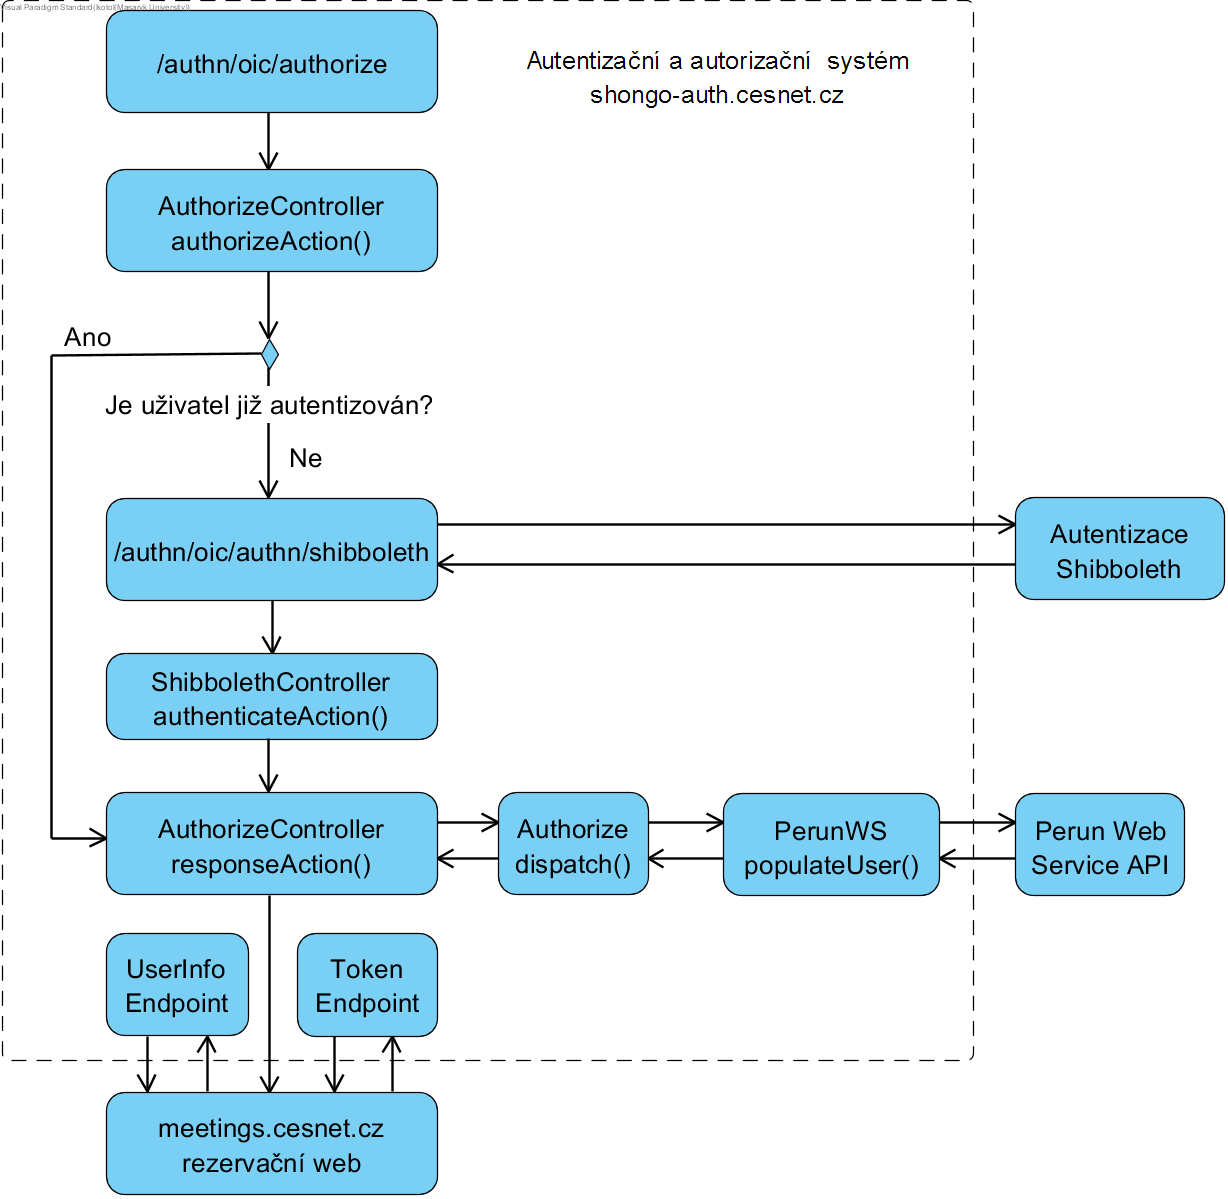
\includegraphics[width=12.8cm]{pics/shongo-auth-layer-old} 
\label{fig:shongoAuthnProcess}
\end{figure}
\par 


\section{Analýza požadavků}
Z konzultací s vedoucím diplomové práce vyplynuly následující požadavky. Jak už bylo uvedeno v úvodu, hlavní podstatou této diplomové práce je vytvoření nové autentizační a autorizační infrastruktury pro videokonferenční a webkonferenční prostředí. Konkrétně se jedná o portály \path{connect.cesnet.cz} a \path{meetings.cesnet.cz} provozované sdružením CESNET pro které bylo zadáno vybudovat novou autentizační a autorizační vrstvu. 

\par
Jedním z hlavních požadavků bylo, aby nová autentizační a autorizační infrastruktura byla navázána na Proxy IdP OpenID Connect, které provozuje sdružení CESNET \cite{proxyIdpPresentation}. Proxy IdP představuje komponentu mezi poskytovatelem služeb a identit, která umožňuje systému aby byl dostupný prostřednictvím různých poskytovatelů identit. 
\par

\par 
Je důležité zmínit, že stávající implementace autentizační a autorizační vrstvy služby \path{meetings.cesnet.cz} je úzce provázána s webovou službou Perun. V rámci ostrého provozu služby \path{meetings.cesnet.cz} byly v minulosti často pozorovány výpadky webové služby Perun. Jelikož se uživatelé při výpadku webové služby Perun nemohly do rezervačního portálu \path{meetings.cesnet.cz} přihlašovat, bylo z důvodu zajištění vyšší dostupnosti portálu \path{meetings.cesnet.cz} požadováno odstranění závislosti na webové službě Perun. 

\par 

Jak bylo v předchozím odstavci zmíněno, webová služba Perun byla ve stávající implementaci provázána s autentizační a autorizační vrstvou rezervačního systému \path{meetings.cesnet.cz}. Konkrétně webová služba Perun zprostředkovávala dodatečné informace o přihlášeném uživateli. Jelikož bylo stanoveno, že v nové implementaci nebude autentizační a autorizační vrstva systému \path{meetings.cesnet.cz} závislá na webové službě Perun, musely být dříve získávané uživatelské údaje pomocí webové služby Perun opatřeny jiným způsobem. Z konzultací s vedoucím této diplomové práce vyplynulo, že zmíněné uživatelské údaje budou v nové implementaci získávány prostřednictvím autorizačního serveru poskytovatele OpenID Connect, který je součástí infrastruktury CESNETu.     

\par

Neméně důležitým požadavkem bylo, aby implementace byla z důvodu centralizace autentizační a autorizační infrastruktury integrována do serveru \path{shongo-auth.cesnet.cz}, na kterém se nachází stávající implementace. 

\section{Návrh nové autentizační a autorizační infrastruktury}
Zde se budu věnovat otázce, jakým způsobem je koncipován návrh nové autentizační a autorizační infrastruktury pro systémy Adobe Connect a \path{meetings.cesnet.cz}. Je vhodné zmínit, že návrh nové autentizační a autorizační architektury pro oba systémy navazuje na architekturu stávající. 

\subsection{Autentizační vrstva systému Adobe Connect}
Nová autentizační a autorizační vrstva webkonferenčního systému Adobe Connect bude využívat již existující implementaci a bude s ní úzce svázána. To znamená, že bude dodána implementace do stávajícího autentizačního serveru \path{shongo-authn.cesnet.cz}. Jak už bylo uvedeno výše, stávající autentizační a autorizační vrstva využívá systému Shibboleth, který bude v rámci této diplomové práce nahrazen implementací systému OpenID Connect. To znamená, že bude muset být systém OpenID Connect a moduly na straně autentizačního serveru \path{shongo-authn.cesnet.cz} do sebe vhodným způsobem integrovány. Tuto skutečnost dosáhneme řádnou instalací autentizačního modulu OpenID Connect webového serveru Apache na autentizační server. Dále musíme zajistit, aby došlo k přemapování atributů získaných po autentizaci uživatele. Implementaci představeného návrhu autentizační vrstvy popisuji v kapitole \hyperref[ACImpl]{4.2}. 

\subsection{Autentizační a autorizační vrstva systému meetings.cesnet.cz}
\label{shong-proposal}
Obdobně jako v případě systému Adobu Connect, bude nová implementace autentizace a autorizace uživatelů do systému \path{meetings.cesnet.cz} úzce propojena se stávající implementací. Jak už bylo uvedeno výše, stávající implementace se nachází na serveru \path{shongo-auth.cesnet.cz}. Je důležité zmínit, že prostřednictvím konfigurace webového serveru Apache budou muset být definovány URL adresy, jejichž použití vyžaduje autentizaci. Jde o URL adresy, které budou vyžadovat delegovanou autentizaci prostřednictvím autorizačního serveru OpenID Connect v Proxy IdP infrastruktuře CESNETu. V rámci konfigurace webového serveru Apache dojde k nastavení modulu podporujícího spolupráci s autorizačním servrem OpenID Connect.  \par

V další fázi bude následovat implementace algoritmu, který zajistí napojení serveru \path{shongo-auth.cesnet.cz} na autorizační server OpenID Connect. Uvedená implementace zajistí mapování nově získaných uživatelských atributů do stávajícího mechanizmu autentizace a autorizace uživatele. Je vhodné zmínit, že dříve proces získání uživatelských atributů byl prováděn pomocí webové služby Perun. Jelikož v nynější implementaci nebude autentizační a autorizační vrstva využívat webovou službu Perun, budou muset být uživatelské atributy získávány prostřednictvím technologie OpenID Connect. Tento mechanizmus bude realizován pomocí nově vytvořeného datového konektoru, jenž se bude nazývat OIDC. Je důležité poznamenat, že nová implementace autorizačního algoritmu zachová nezbytnou kontrolu příslušnosti uživatele do skupiny einfra. 
\par

Dalším krokem je adaptace systému \path{meetings.cesnet.cz} na provedené změny v rámci implementace na straně serveru \path{shongo-auth.cesnet.cz}. Tuto adaptaci představují tři klíčové body. 

\par 

Prvním z nich je nahrazení identifikátoru uživatele \textbf{perun id} za \textbf{einfra id}. Zmíněné identifikátory jednoznačně identifikují uživatele v rámci webové služby Perun, respektive v OpenID Connect infrastruktuře CESNETu. Nutnost nahrazení identifikátorů vychází z toho, že autorizační server OpenID Connect v infrastruktuře CESNETu neposkytuje identifikátor \textbf{perun id} v rámci svých \textbf{Claims}. Jelikož ve stávající implementaci systému \path{meetings.cesnet.cz} se při jakékoliv práci s uživatelem využívá identifikátor \textbf{perun id}, bude muset být tento identifikátor vhodným způsobem nahrazen. Zmíněná náhrada identifikátorů \textbf{perun id} za \textbf{einfra id} bude muset být provedena jak pro všechny stávající uživatele uložené v databázi, tak pro všechny budoucí uživatele využívající systém \path{meetings.cesnet.cz}. Je důležité zmínit, že k úspěšnému nahrazení identifikátoru \textbf{perun id} za \textbf{einfra id} bude muset být zvětšena velikost sloupce tabulky v databázi, uchovávající uvedený identifikátor. Představená změna velikosti sloupce musí být provedena z toho důvodu, jelikož stávající velikost sloupce by nedostačovala nahrazovanému identifikátoru \textbf{einfra id}. 
\par

Druhým bodem je nutnost uložení dodatečných informací o autentizovaném uživateli do databáze systému \path{meetings.cesnet.cz}. Zmíněná data jsou ve stávající implementaci získávána při každém požadavku na zobrazení uživatelských informací pomocí webové služby Perun. Jelikož nová implementace nebude závislá na webové službě Perun, musí se představené uživatelské informace ukládat do databáze již v rámci procesu autentizace uživatele. Uvedená modifikace implikuje další změnu, a to že bude muset být vytvořen algoritmus, který do databáze systému \path{meetings.cesnet.cz} uloží uživatelské informace všech stávajících uživatelů. Obdobným způsobem bude odstraněna vazba na správu skupin pomocí webové služby Perun. Díky odstranění závislosti autentizační a autorizační vrstvy na webové službě Perun dojde k nemalé snížení složitosti stávajících systémů. 
\par 

Posledním bodem je modifikace samotného zdrojového kódu systému Shongo, který je nasazen na URL adrese \path{meetings.cesnet.cz}. Ta se bude sestávat z adaptace na změnu URL adresy autentizačního, Token a UserInfo Endpointů. Dále bude pozměněna kontrola příslušnosti uživatele do skupin, na základě které je uživateli umožněno využívat zdroje. Uvedená kontrola dříve využívala volání webové služby Perun, v nové implementaci bude se budou získávat potřebné informace o příslušnosti uživatele do skupin z UserInfo Endpointu. V neposlední řadě bude provedena modifikace logické vrstvy systému \path{meetings.cesnet.cz}. Ta bude spočívat v pozměnění metod, tak aby získavaly požadovaná data z databáze, místo vytváření HTTP požadavků na webovou službu Perun. 

\par 

Je vhodné dodat, že v rámci této diplomové práce nebude modifikována prezentační vrstva, jelikož nemá žádnou souvislost koncipovaným návrhem nové autentizační a autorizační vrstvy rezervačního systému \path{meetings.cesnet.cz}.

\par

Implementaci představených změn v autentizační a autorizační vrstvě systému \path{meetings.cesnet.cz} popisuji v kapitole \hyperref[ShongoImpl]{4.3}.

\chapter{Použité technologie}
V této kapitole popisuji technologie, které jsem použil při implementaci diplomové práce. Popis doplňuji informací o tom, v které konkrétní části implementace jsem danou technologii použil.
\section{OAuth}
\label{sec:oauth}
OAuth 2.0 \cite{rfc6749} je autorizační framework, který umožňuje aplikacím třetí strany získat omezený přístup k HTTP službám. Tento framework je tedy určen pro bezpečné delegování přístupu. Zmíněný framework představuje autorizační vrstvu, která odděluje role klienta od držitele zdrojů. Specifikace OAuth 2.0 popisuje následující role: 
\begin{itemize}
    \item \textbf{Resource Owner} je entita, schopná dát souhlas s přístupem k požadovanému zdroji, většinou koncový uživatel,
    \item \textbf{Resource Server} představuje server, uchovávající chráněné zdroje, schopný odpovídat požadavkům přistupujícím k chráněným zdrojům,
    \item \textbf{Client} je aplikace, vytvářející požadavky na získání chráněných zdrojů se svolením role \textbf{Resource Owner},
    \item \textbf{Authorization Server} je server, vydávající \textbf{Access Token} pro roli \textbf{Client} po úspěšném ověření identity \textbf{Resource Owner} a získání oprávnění.
\end{itemize}
Uvedený pojem \textbf{Access Token} je pověření používané k získání přístupu k chráněným zdrojům. \textbf{Access Token} se obvykle vydává ve formátu \textbf{JWT (JSON Web Token)}. Formátu \textbf{JWT} se věnuji v následující sekci v kapitole \hyperref[sec:oidc]{3.2}.  \par

Schéma komunikace v protokolu OAuth 2.0 ilustruje následující obrázek \hyperref[fig:oauth]{3.1}. 

\begin{figure}[H]
\caption{Schéma komunikace v protokolu OAuth 2.0}
\centering
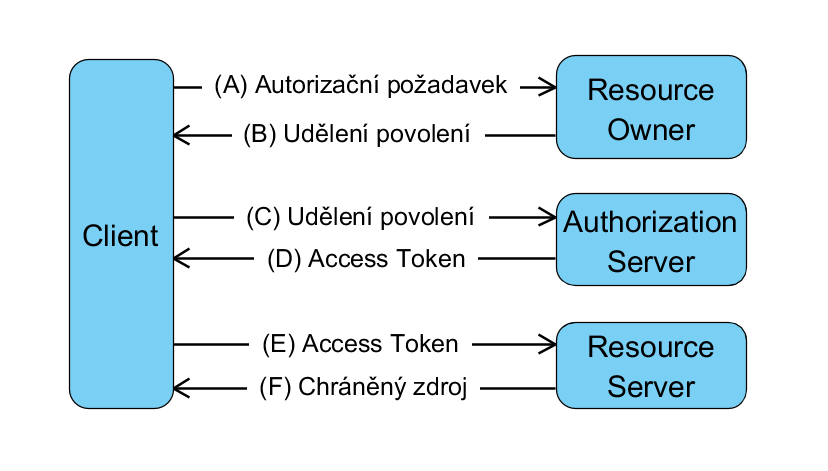
\includegraphics[width=12.8cm]{pics/diplomkaOauth} 
\label{fig:oauth}
\end{figure}
\par 

V prvním kroku (A) \textbf{Client} požaduje autorizaci po \textbf{Resource Owner}. V další fázi (B) \textbf{Client} získá pověření, které představuje oprávnění vlastníka k přístupu ke zdrojům. V následujícím kroku (C) \textbf{Client} požaduje \textbf{Access Token} po \textbf{Authorization Server}, kterému prezentuje udělená oprávnění. Další krok (D) představuje autentizaci a validaci uděleného oprávnění, na základě jehož je vydán \textbf{Access Token}. V předposlední fázi (E) \textbf{Client} přistupuje k \textbf{Resource Server} s \textbf{Access Tokenem} a požadavkem na získání chráněného zdroje. Po validaci \textbf{Access Tokenu} poskytne \textbf{Resource Server} požadované zdroje entitě \textbf{Client} (F). \par 

Autorizační protokol OAuth 2.0 není navržen pro autentizaci uživatelů a neposkytuje možnost získání dalších informací o přihlášeném uživateli. Z těchto důvodů byl protokol OAuth 2.0 v implementaci použit spolu s technologií OpenID Connect, která zmíněnou funkcionalitu definuje a umožňuje ji vhodně implementovat. 

\section{OpenID Connect}
\label{sec:oidc}
OpenID Connect 1.0 \footnote{Dokumentace OpenID Connect 1.0, \url{www.openid.net/specs/openid-connect-core-1_0.html}} je protokol, který umožňuje aplikaci verifikovat identitu uživatele na základě autentizace provedené autorizačním serverem. Jedná se o autentizační vrstvu nad frameworkem OAuth 2.0. Důležitou vlastností OpenID Connect je definice způsobu získaní základních informací o přihlášeném uživateli. \par

Hlavním rozšířením protokolu OpenID Connect oproti OAuth 2.0 umožňující autentizaci je definice nové datové struktury \textbf{ID Token}. Uvedený \textbf{ID Token} je bezpečnostní žeton, který obsahuje informace o autentizaci a případná další doplňková data koncového uživatele. Zmíněné informace nacházející se ve struktuře \textbf{ID Token} nazývají v tomto kontextu \textbf{Claims}. Popisované \textbf{Claims} vždy nesou informace ve formátu dvojice název \textbf{Claim} a hodnota \textbf{Claim}. Představované \textbf{Claims}, které uchovávají informace o autentizované entitě, jsou ve struktuře \textbf{ID Token} zakódovány ve formátu \textbf{JWT} (JSON Web Token) \cite{rfc7519}.    

\par

\textbf{JWT} je textový řetězec reprezentující \textbf{Claims} jako JSON objekt \cite{rfc8259}  zakódovaný pomocí Base64 \cite{rfc4648} kódování a HMAC s SHA-256 \cite{rfc4868}. Popisovaný \textbf{JWT} je standardně rozdělen na části hlavičku a tělo. Po aplikaci algoritmů Base64 a HMAC s SHA-256 na tyto dvě části se vytvoří výsledný řetězec. Konkrétní mechanizmus způsobu vytváření \textbf{JWT} je detailně popsán v odkazovaném RFC 7519 \cite{rfc7519}. \par

Protokol OpenID Connect dále definuje jaké \textbf{Claims} musí struktura \textbf{ID Token} obsahovat:

\begin{itemize}
    \item \textbf{iss} představuje identifikátor entity, která vytvořila \textbf{ID Token}, 
    \item \textbf{sub} označuje identifikátor autentizovaného uživatele, 
    \item \textbf{aud} je pole identifikátorů entit, pro které je vydaný \textbf{ID Token} určen,
    \item \textbf{exp} reprezentuje časový údaj, do kdy je vydaný \textbf{ID Token} platný
    \item \textbf{iat} označuje informaci, kdy byl \textbf{ID Token} vydán.
\end{itemize}
\par

Před samotným rozborem schématu komunikace v protokolu OpenID Connect je vhodné definovat následující pojmy. \textbf{OpenID Provider (OP)} představuje autorizační server schopný autentizovat koncového uživatele. Jednou z klíčových funkcí \textbf{OP} je možnost poskytnout \textbf{Relying Party} \textbf{Claims} o autentizační události a autentizovaném uživateli. Zmíněný pojem \textbf{Relying Party (RP)} označuje klientskou aplikaci, požadující autentizaci uživatele a \textbf{Claims} od \textbf{OP}. \par
Následující obrázek \hyperref[fig:oidc]{3.2} popisuje s použitím dříve definovaných pojmů schéma komunikace v protokolu OpenID Connect.

\begin{figure}[H]
\caption{Schéma komunikace v protokolu OpenID Connect 1.0}
\centering
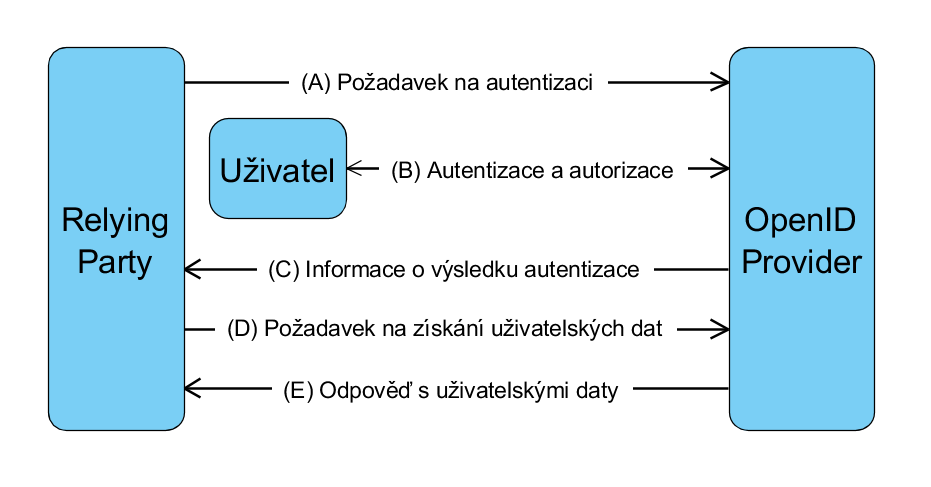
\includegraphics[width=12.8cm]{pics/diplomkaOIDC} 
\label{fig:oidc}
\end{figure}
\par 

V první fázi (A) pošle \textbf{Relying Party} autentizační požadavek autorizačnímu serveru \textbf{OpenId Provider}. V dalším kroku (B) \textbf{OP} autentizuje koncového uživatele a provede autorizaci. V třetí fázi (C) odpoví autorizační server \textbf{OP} na požadavek informací o výsledku autentizace spolu s žetony \textbf{ID Token} a \textbf{Access Token}. V dalším kroku (D) \textbf{RP} může pomocí \textbf{Access Tokenu} poslat \textbf{OP} požadavek na získání uživatelských dat. Nakonec poslední fází (E) komunikačního schématu je odpověď \textbf{OP} s \textbf{Claims} obsahující uživatelská data, které si v předchozím kroku \textbf{RP} vyžádal. 
\par

V předchozím odstavci je zmíněna předposlední fáze \textbf{D} ve které \textbf{RP} po autentizaci posílá požadavek \textbf{OP} na získání dat o uživateli. Zdroj, který tyto informace uchovává se nazývá \textbf{UserInfo Endpoint}. Představovaný \textbf{UserInfo Endpoint} je chráněná URL adresa, která akceptuje HTTP požadavky pouze s přiloženým validním \textbf{Access Tokenem}. Formát odpovědi a požadované \textbf{Claims}, které \textbf{UserInfo Endpoint} poskytuje se nastavují při registraci \textbf{OpenID Providera}. Je vhodné doplnit, že ve fázi, kdy při registraci \textbf{OpenID Providera} definujeme požadované \textbf{Claims}, tak pracujeme raději s pojmem \textbf{Scopes}. Představené \textbf{Scopes} tedy indikují údaje o uživateli, ke kterým bude chtít registrovaný klient po úspěšné autentizaci přistupovat.
\par

Jak už bylo zmíněno v sekci která se věnuje popisu stávající implementace systému \path{meetings.cesnet.cz}, proces autentizace a autorizace je řízen pomocí tzv. Authorization Code flow. Tento způsob získání \textbf{ID Tokenu} a \textbf{Access Tokenu} vkládá do popisovaného komunikačního schématu v protokolu OpenID Connect další fázi. Místo zmíněných žetonů je v kroku (C) autorizačním serverem \textbf{OP} vrácen vygenerovaný textový řetězec tzv. \textbf{Authorize code}. Tento \textbf{Authorize code} je v následujícím kroku vyměněn za požadované žetony \textbf{ID Token} a \textbf{Access Token}. Podobně jako v případě \textbf{UserInfo Endpoint}, chráněný zdroj na straně autorizačního serveru \textbf{OP}, který poskytuje žetony na základě validace \textbf{Authorize code} se nazývá \textbf{Token Endpoint}.

\par
OpenID Connect je klíčová technologie, který byla využita při vypracování této diplomové práce k vytvoření nové autentizační a autorizační infrastruktury. Existuje velké množství certifikovaných implementací technologie OpenID Connect v mnoha různých programovacích jazycích\footnote{Certified OpenID Connect implementations, \url{www.openid.net/developers/certified/}}. V této diplomové práci jsem použil MITREid Connect\footnote{MITREid Connect, \url{www.mitreid-connect.github.io/}}, jelikož je již integrována v infrastruktuře CESNETu jako implementace OpenID Connect \cite{oidcPresentation}. Jedná se o webovou aplikaci napsanou v programovacím jazyce Java, která je založená na frameworku Spring Security\footnote{Spring Security framework documentation, \url{www.docs.spring.io/spring-security/site/docs/current/reference/htmlsingle/}}. 

\section{Ostatní technologie}
V této kapitole popisuji další technologie, které jsem využil v rámci implementace autentizační a autorizační infrastruktury. 
\par
Jednou z hlavních technologií, kterou jsem použil při vypracování této diplomové práce je webový server Apache. Ústředním modulem, který slouží pro integraci s poskytovatelem OpenID Connect je \textbf{mod\_auth\_openidc}\footnote{Apache modul mod\_auth\_openidc, \url{https://github.com/zmartzone/mod\_auth\_openidc}}. Zmíněný modul umožňuje autentizovat a autorizovat klientskou aplikaci vůči autorizačnímu serveru OpenID Connect. Modul dále může sloužit i pro nastavení serveru, který funguje jako tzv. \textbf{Resource Server} v rámci protokolu OAuth 2.0. Konkrétní způsob konfigurace Apache spolu s OpenID Connect modulem popisuji v kapitole \hyperref[apacheConfig]{4.1}.

\par
Další klíčovou technologií, kterou jsem při práci využil je programovací jazyk PHP. V uvedeném programovacím jazyce jsem na straně serveru \path{shongo-auth.cesnet.cz} implementoval autentizační a autorizační logiku. Architektura serveru \path{shongo-auth.cesnet.cz} starající se o autentizaci a autorizaci uživatelů je vystavěna na aplikačním frameworku Zend \cite{zend}. Zmíněná implementace je detailněji popsána v kapitolách \hyperref[ACImpl]{4.2}, \hyperref[ShongoImpl-authn]{4.3.1} a \hyperref[ShongoImpl-authr]{4.3.2}. 

\par

Další technologií, kterou jsem při při vývoji nové autentizační a autorizační infrastruktury použil je databázový server PostgreSQL. S PostgreSQL jsem pracoval při adaptaci databáze systému \path{meetings.cesnet.cz} na provedené v změny autentizační a autorizační vrstvě. Zmíněná adaptace sestávala z následujících dílčích kroků. Prvním bylo nahrazení primárního klíče uživatele z \textbf{perun id} na unikátní identifikátor uživatele  \textbf{einfra id} v rámci infrastruktury OpenID Connect CESNETu. Další krok tvořil vkládání dodatečných informací o stávajících uživatelích rezervačního systému \path{meetings.cesnet.cz}. V neposlední řadě jsem představený databázový server využil při modifikaci stávajícího schématu databáze systému \path{meetings.cesnet.cz}. Tyto operace detailněji popisuji v kapitole \hyperref[ShongoImpl]{4.3}. 
\par 
Posledními významnými technologiemi, které jsem využil při vypracování této diplomové práce jsou programovací jazyk Java a objektově relační framework Hibernate \footnote{Hibernate ORM framework , \url{www.hibernate.org/orm/}}. Jedná se o technologie, které jsou použity ve stávající implementaci rezervačního systému Shongo a využil jsem je při integraci s novou autentizační a autorizační vrstvou.  


\chapter{Popis implementace}
V této kapitole seznamuji s detailním postupem při implementaci a instalaci nové autentizační a autorizační infrastruktury využívající protokol OpenID Connect. V kapitole \hyperref[apacheConfig]{4.1} popisuji jakým způsobem probíhala instalace a konfigurace modulu OpenID Connect pro webový server Apache. V dalších kapitolách \hyperref[ACImpl]{4.2} a \hyperref[ShongoImpl]{4.3} se věnuji implementaci autentizační a autorizační vrstvy systému Adobe Connect, respektive systému Shongo.   


\section{Instalace a konfigurace Apache modulu pro OpenID Connect}
\label{apacheInstall}
V této kapitole popisuji instalaci a konfiguraci Apache modulu pro OpenID Connect. Dále se věnuji registraci klienta \path{shongo-auth.cesnet.cz} do Proxy IdP infrastruktury CESNETu. Zmíněné operace byly provedeny podle pokynů dostupných v prezentaci prezentované na dnech s Perunem \cite{oidcConfigPresentation}.

\label{apacheConfig}
\subsection{Instalace knihoven modulu mod\_auth\_openidc}
Instalace knihoven nutných pro zprovoznění Apache modulu OpenID Connect byly v rámci diplomové práce prováděny na serveru \path{shongo-auth.cesnet.cz} s operačním systémem Debian GNU/Linux 7 (wheezy). 
\par 
Autentizační a autorizační modul, který slouží pro zprovoznění serveru jako tzv. \textbf{OpenID Connect Relying Party} se nazývá \linebreak \textbf{mod\_auth\_openidc\footnote{OpenID Connect Relying Party pro Apache server \url{https://github.com/zmartzone/mod\_auth\_openidc}}}. Důležitým předpokladem pro instalaci představeného modulu je již dříve nainstalovaný server Apache. Apache se na serveru \path{shongo-auth.cesnet.cz} již nachází a tudíž jej nebylo nutné instalovat. 
\par 
Prvním krokem, který jsem provedl byla instalace nezbytných knihoven \textbf{libjansson4} a \textbf{libhiredis0.13}, \textbf{libcjose0\_0.5} a \textbf{libapache2-mod-auth-openidc\_2.3.3-1}. Po instalaci uvedených knihoven následovala registrace klienta do Proxy IdP infrastruktury. 

\subsection{Registrace klienta do Proxy IdP infrastruktury}

Po úspěšně dokončené instalaci uvedených knihoven následovala registrace klienta \path{shongo-auth.cesnet.cz} do Proxy IdP infrastruktury sdružení CESNET. Zmíněná registrace probíhala ve webové aplikaci MITREid Connect dostupné na adrese \url{https://login.cesnet.cz/oidc/}. Po přihlášení do webové aplikace bylo prostřednictvím uživatelského rozhraní v levém menu v kolonce \textbf{Developer} vybrán odkaz \textbf{Self-service client registration}. Uvedená akce přesměrovala prohlížeč na stránku s tlačítkem \textbf{New Client} sloužící pro registraci nového klienta. Po kliknutí na zmíněné tlačítko aplikace přesměrovala prohlížeč na registrační formulář s konfigurací nového klienta. V záložce \textbf{Main} byla vyplněna kolonka \textbf{Redirect URI(s)} adresou \path{https://shongo-auth.cesnet.cz/oauth2callback}. Uvedená kolonka představuje URL adresu pro přesměrování po autentizaci koncového uživatele. Dále byly vyplněny údaje v záložce \textbf{Access} v kolonce \textbf{Scope}. Zmíněné \textbf{Scopes} indikují údaje o uživateli, ke kterým bude chtít registrovaný klient po autentizaci přistupovat. Je vhodné v kontextu \textbf{Scopes} zmínit i další pojem \textbf{Claims}, což značí již konkrétní uživatelské údaje ve formátu dvojice klíč a hodnota. V rámci registrace klienta byly tedy vybrány následující \textbf{Scopes}.

\begin{itemize}
    \item \textbf{openid} představuje unikátní identifikátor uživatele v rámci Proxy IdP ifrastruktury, tzv. einfra id,
    \item \textbf{profile} jde o osobní profil uživatele požadující \textbf{Claims} \textbf{name}, \textbf{given\_name}, \textbf{middle\_name}, \textbf{family\_name}, \textbf{preferred\_username}, \textbf{zoneinfo} a \textbf{locale},
    \item \textbf{email} označuje emailovou adresu uživatele,
    \item \textbf{address} je poštovní adresa uživatele,
    \item \textbf{phone} odkazuje na telefonní číslo uživatele,
    
    \item \textbf{organization} představuje domovskou organizaci ke které uživatel patří,
    \item \textbf{eppns} značí seznam všech \textbf{eduPersonPrincipalName} uživatele, jde o jednoznačné identifikátory v rámci federace, mající formát uživatelské\_jméno@doména,  
    \item \textbf{eduPersonEntitlement} obsahuje seznam skupin, kterých je uživatel členem a jsou na službu \path{meetings.cesnet.cz} přiřazeny.
    
\end{itemize}
Dále je důležité zmínit, že v kolonce \textbf{Grant Types} byl zvolen \textbf{authorization code}, který respektuje nastavení předávaní tokenů v protokolu OpenID Connect v autentizační a autorizační architektuře registrovaného serveru \path{shongo-auth.cesnet.cz}.  \par

Po uložení zmíněné konfigurace byly aplikací náhodně vygenerovány tyto následující údaje. Jde o \textbf{Client ID}, které jednoznačně identifikuje registrovaného klienta \path{shongo-auth.cesnet.cz}. Dále byl vygenerován registrační token, tzv. \textbf{Registration Access Token}, který slouží pro pozdější zpřístupnění editace konfigurace vytvořeného klienta. Posledním údajem, který byl vygenerován je sdílené tajemství mezi klientskou aplikací a autorizačním serverem, tzv. \textbf{Client Secret}. Zmíněný \textbf{Client Secret} autentizuje požadavky klientské aplikace vůči autorizačnímu serveru. Vygenerované údaje jsem dále využil v rámci konfigurace modulu mod\_auth\_openidc, kterou popisuji v následující sekci \hyperref[sec:mod-conf]{4.1.3}.

\subsection{Konfigurace Apache modulu mod\_auth\_openidc} 
\label{sec:mod-conf}
Předpokladem pro kompletní zprovoznění OpenID Connect modulu je spuštění příkazu \path{a2enmod auth_openidc} který zapnul tento dříve nainstalovaný modul. Potom následovalo nastavení nainstalovaného modulu v konfiguračním souboru Apache serveru \path{/etc/apache2/sites-available/default-ssl}. Do zmíněného souboru jsem přidal následující konfigurace.

\begin{itemize}
    \item \textbf{LoadModule auth\_openidc\_module /usr/lib/apache2\\ /modules/mod\_auth\_openidc.so} značí načtení požadovaného OpenID Connect modulu, 
    \item \textbf{OIDCProviderMetadataURL https://login.cesnet.cz/oidc/.well-known/openid-configuration} představuje adresu odkazu na konfiguraci poskytovatele OpenID Connect, 
    \item \textbf{OIDCProviderMetadataRefreshInterval 3600} definuje nastavení intervalu pro obnovení metadat poskytovatele OpenID Connect, 
    \item \textbf{OIDCClientID \{Client ID\}} nastavuje identifikaci klienta, tato hodnota byla vygenerovaná v rámci registrace,
    \item \textbf{OIDCClientSecret \{Client Secret\}} definuje sdílené tajemství mezi klientem a poskytovatelem OpenID Connect, také se použije hodnota, která byla dříve vygenerovaná při registraci,
    \item \textbf{OIDCScope "openid email profile address phone organization eppns eduPersonEntitlement"} slouží pro nastavení \textbf{Scopes}, které jsou požadované od poskytovatele OpenID Connect, vyčet \textbf{Scopes} odpovídá zvoleným \textbf{Scopes} při registraci klienta do Proxy IdP infrastruktury,
    \item \textbf{OIDCRedirectURI /oauth2callback} značí adresu na kterou bude prohlížeč přesměrován po autentizaci, musí mít stejnou hodnotu jako zvolená hodnota při registraci klienta, 
    \item \textbf{OIDCCryptoPassphrase \{heslo\}} představuje heslo pro šifrování cookie a cache dat. 
\end{itemize}

Po nastavení uvedené konfigurace, mohlo dojít ke stanovení URL adres, které při přístupu požadují OpenID Connect autentizaci. Zmíněnou ochranu adres pro autentizační a autorizační vrstvu Adobe Connect jsem definoval pomocí Apache direktiv \textbf{Location}, \textbf{AuthType} a \textbf{Require}. Pro pochopení, jakým způsobem jsem nakonfiguroval Apache server je vhodné si vysvětlit význam použitých direktiv. Direktiva \textbf{Location} definuje rozsah použité konfigurace pomocí URL. Další direktiva \textbf{AuthType} značí požadovaný typ autentizace, v tomto případe jde o protokol OpenID Connect. Poslední direktiva \textbf{Require} představuje nastavení, požadující při přístupu na zvolenou URL adresu validně přihlášeného uživatele. Následuje výňatek z konfiguračního souboru Apache, který ilustruje požadovanou ochranu URL adres autentizační a autorizační vrstvu Adobe Connect.
\begin{lstlisting}
          <Location /oidc-ac>
                  AuthType openid-connect
                  Require valid-user
          </Location>
\end{lstlisting}
\label{ac-location}

Obdobně ochranu URL adres mapovaných na moduly, které se starají o autentizaci a autorizaci uživatelů přistupujících na server \path{meetings.cesnet.cz} zajišťuje následující úryvek. 

\begin{lstlisting}
          <Location /oidc-authn/oic/authn/oidc>
                  AuthType openid-connect
                  Require valid-user
          </Location>
          
          <Location /oidc-authn/oic/authorize-response>
                  AuthType openid-connect
                  Require valid-user
          </Location>
\end{lstlisting}
První představená URL adresa \path{/oidc-authn/oic/authn/oidc} je mapována na nově vytvořenou třídu \path{OIDCController}, která se stará o zprostředkování autentizace. Druhá URL adresa \path{/oidc-authn/oic/authorize-response} slouží po autentizaci k zpřístupnění získaných \textbf{Claims} o uživateli. Dalšímu použití  chráněných URL adres se věnuji v rámci popisu implementace autentizační a autorizační vrstvy systému \path{meetings.cesnet.cz} v kapitolách \hyperref[ShongoImpl-authn]{4.3.1} a \hyperref[ShongoImpl-authn]{4.3.2}.

\label{shongo-location}

\section{Implementace autentizační vrstvy systému Adobe Connect}
\label{ACImpl}
V této sekci se zabývám popisem implementace, kterou bylo nutné provézt při integraci stávající autentizační vrstvy systému Adobe Connect s OpenID Connect Proxy IdP provozované sdružením CESNET. 
\par 
Pro pochopení provedených změn je důležité připomenou ústřední prvky stávající implementace. V stávající implementaci jsou uživatelské atributy po autentizaci prostřednictvím systému Shibboleth mapovány na objekt představujícího uživatele. Dále je důležité zmínit, že jednou z hlavní částí této diplomové práce je nahrazení autentizačního systému Shibboleth za implementaci protokolu OpenID Connect. Jelikož autentizační modul Apache \textbf{mod\_auth\_openidc} zprostředkuje atributy autentizovaného uživatele odlišným způsobem než aktuální konfigurace sytému Shibboleth, bylo klíčové zajistit přemapování zmíněných uživatelských atributů. Popis konfigurace a instalace zmíněného modulu \textbf{mod\_auth\_openidc} je představen v kapitole \hyperref[apacheInstall]{4.1}.  
\par

Popsané přemapování uživatelských atributů bylo provedeno v konfiguračním souboru \path{config/connect.ini} autentizační vrstvy. Následující výňatek konfiguračního souboru popisuje nové mapování uživatelských atributů do proměnných autentizačního algoritmu. 

\begin{lstlisting}[
    basicstyle=\footnotesize\ttfamily,
    columns=fullflexible,
    commentstyle=\color{gray}\ttfamily,
    morekeywords={},
    otherkeywords={=,:},
    keywordstyle={\color{red}\bfseries},
    backgroundcolor=\color{background},
    frame=lines
]
uid_field = OIDC_CLAIM_sub
eppns_field = OIDC_CLAIM_eppns
mail_field = OIDC_CLAIM_email
givenName_field = OIDC_CLAIM_given_name
sn_field = OIDC_CLAIM_family_name
\end{lstlisting}
První řádek výňatku mapuje unikátní identifikátor einfra id, druhý řádek seznam obsahující \textbf{eduPersonPrincipalName}, další řádek emailovou adresu, předposlední řádek jméno a poslední řádek příjmení uživatele. Atribut \textbf{eppns\_field} značí uživatelské identifikátory v jednotlivých organizacích, kterých je uživatel členem. Uvedené atributy jsou v autentizačním algoritmu nastaveny objektu představujícího uživatele. 
\par 

Se zmíněným objektem představujícího přihlašovaného uživatele se dále pracuje, tak jako ve stávající implementaci. To znamená že je provedena kontrola, zda uživatel již existuje v interní databázi webkonferenčního systému Adobe Connect. Protože ve stávající implementaci atribut \textbf{eppns\_field} obsahoval pouze jedno \textbf{eduPersonPrincipalName}, kontrolovala se existence pouze jednoho přítomného identifikátoru v databázi. Detailní popis představeného procesu kontroly existence uživatele v databázi ve stávající implementaci autentizační vrstvy systému Adobe Connect je uveden v kapitole \hyperref[ac-old]{2.1.1}. V nové implementaci musela být provedena kontrola existence uživatelského identifikátoru \textbf{eduPersonPrincipalName} odlišným způsobem. Příčinou této změny je fakt, že do atributu \textbf{eppns\_field} je nově mapován seznam několika \textbf{eduPersonPrincipalName} místo jediného uživatelského identifikátoru.
\par
Z důvodu popisovaného v předchozím odstavci byla do autentizačního algoritmu přidána metoda \path{_getExistingUserIdByEppns}. Tato metoda najde ze seznamu všech \textbf{eppns\_field} takový identifikátor uživatele, který již v interní databázi Adobe Connect existuje. Pokud metoda \path{_getExistingUserIdByEppns} nenajde žádného uživatele v interní databázi Adobe Connect, vytvoří algoritmus v databázi záznam představujícího uživatele. Zmíněný záznam, je primárně vytvořen z takového \textbf{eduPersonPrincipalName}, které představuje uživatelský identifikátor v rámci skupiny einfra. Popisované \textbf{eduPersonPrincipalName} identifikující uživatele v rámci einfra skupiny má formát \textbf{{uživatelský\_identifikátor}@einfra.cesnet.cz}. Důsledkem příslušnosti uživatele do skupiny einfra je tzv. \textbf{LoA} úrovně dva. \textbf{LoA} (Level of Assurance) \cite{rfc6711} je úroveň záruky vyjadřující míru spolehlivosti prostředků pro
elektronickou identifikaci při určování totožnosti dané osoby. V tomto kontextu \textbf{LoA} úrovně dva značí, že uživatel je schopný ověřit svoji identitu pomocí hesla.  Pokud v krajním případě uživatel nepatří do skupiny einfra je v rámci nové implementace použit první uživatelský identifikátor ze seznamu \textbf{eduPersonPrincipalName}. Dále již běh algoritmu pokračuje obdobně jako ve stávající implementaci autentizační vrstvy systému Adobe Conect, kterou popisuji v kapitole \hyperref[ac-old]{2.1.1}. 


\par 
Nakonec, je důležité poznamenat, že nová implementace autentizační vrstvy systému Adobe Connect byla přesunuta do adresáře \path{/app/oidc/}. Dále je důležité zmínit, že chráněná URL adresa definovaná v \hyperref[ac-location]{konfiguračním souboru} Apache je mapována právě na uvedený adresář \path{/app/oidc/}. Z toho plyne, že nová URL adresa určená pro zpracování GET autentizačních požadavků na přihlášení do webkonferenčního systému Adobe Connect má formát \path{https://shongo-auth.cesnet.cz/oidc-ac/instance/connect}.


\section{Implementace autentizační a autorizační vrstvy systému meetings.cesnet.cz}
\label{ShongoImpl}
V této kapitole se zabývám popisem postupu implementace při integraci stávající autentizační a autorizační vrstvy služby \path{meetings.cesnet.cz} do Proxy IdP provozované sdružením CESNET. V kapitole \hyperref[ShongoImpl-authn]{4.3.1} představuji implementaci autentizační logiky na straně serveru \path{shongo-auth.cesnet.cz}. Další kapitola pojednává o specifikách implementace autorizační vrstvy \hyperref[ShongoImpl-authr]{4.3.2}. V další kapitole \hyperref[zpracovaniAUlozeniPerun]{4.3.3} se věnuji popisu odstranění závislosti datové vrstvy systému \path{meetings.cesnet.cz} na webové službě Perun. Kapitola \hyperref[ShongoImpl-web]{4.3.4} pojednává o implementačních změnách v logické vrstvě rezervačního systému Shongo, provozovaného na URL adrese \path{meetings.cesnet.cz}. 

\subsection{Implementace autentizační logiky na serveru shongo-auth.cesnet.cz}
\label{ShongoImpl-authn}    

Zde se věnuji popisu implementace algoritmu, který zajišťuje autentizaci klienta \path{shongo-auth.cesnet.cz} vůči autorizačnímu serveru OpenID Connect v infrastruktuře CESNETu.  

\par

Jak vyplynulo ze zadání diplomové práce, klíčovou součástí implementace je vytvoření nové autentizační vrstvy systému \path{meetings.cesnet.cz}.
\par

Jednou z hlavních částí zmíněné implementace je nahrazení funkcionality stávajícího autentizačního systému Shibboleth za OpenID Connect poskytovatele.
Je důležité zmínit, že o samotnou autentizaci uživatelů se stará konkrétní poskytovatel identit ve spolupráci s autorizačním server OpenID Connect. Delegování autentizace je jednou ze základních vlastností protokolu OpenID Connect a zprovoznění této funkcionality bylo dosaženo řádnou instalací Apache modulu \textbf{mod\_auth\_openidc} a registrací klienta \path{shongo-auth.cesnet.cz} do Proxy IdP infrastruktury CESNETu. Proto je samotná autentizace přenechána poskytovatelům identit a není již řešena na straně serveru \path{shongo-auth.cesnet.cz}. Uvedené řešení respektuje stávající architekturu, která dříve obdobným způsobem využívala k autentizaci uživatelů systém Shibboleth. 

\par 
Dalším krokem vykonaným v rámci implementace nové autentizační a autorizační vrstvy bylo nahrazení funkcionality webové služby Perun.  
Jelikož autentizační algoritmus na straně serveru \path{shongo-auth.cesnet.cz} počítá s uživatelskými atributy získanými ze systémů Shibboleth a Perun, muselo dojít k vhodnému přemapování těchto atributů. Systém Shibboleth poskytoval pouze podmnožinu uživatelských atributů, něž jakou poskytuje webová služba Perun, a tudíž stačilo v tomto kontextu nahradit pouze funkcionalitu zmiňované webové služby Perun. \par

Jak již bylo představeno v popisu stávající autentizační a autorizační logiky systému \path{shongo-auth.cesnet.cz}, volání webové služby Perun se realizují v datovém konektoru PerunWS. Hlavní úkolem tohoto datového konektoru je získání a zpracování dat z webové služby Perun do objektu představujícího uživatele. Zmíněný datový konektor jsem nahradil novým datovým konektorem, který zpracovává uživatelské údaje po autentizaci prostřednictvím poskytovatele OpenID Connect. Úkolem uvedeného datového konektoru je zpracování uživatelských atributů dostupných v globální proměnné prostředí \path{$_SERVER}. Je důležité zmínit, že uživatelské atributy jsou po autentizaci uživatele do proměnné \path{$_SERVER} zprostředkovány díky dříve nainstalovanému Apache modulu \textbf{mod\_auth\_openidc}. Abychom mohli představené uživatelské atributy zpracovat, byl vytvořen soubor \path{OIDC.php}, který reprezentuje zmíněný datový konektor. Vytvořený konektor \path{OIDC.php} plně nahrazuje konektor \path{PerunWS.php}, který v předcházející implementaci získával informace o přihlášeném uživateli pomocí webové služby Perun. Nově vytvořený konektor mapuje následující atributy v poli \path{$_SERVER} do objektu představujícího autentizovaného uživatele \path{ShongoAuthn\User\User}. 

\begin{itemize}
    \item \textbf{OIDC\_CLAIM\_sub} značí unikátní identifikátor uživatele v infrastruktuře CESNETu, tzv. einfra id,
    \item \textbf{OIDC\_CLAIM\_given\_name} představuje křestní jméno uživatele,
    \item \textbf{OIDC\_CLAIM\_family\_name} obsahuje příjmení uživatele,
    \item \textbf{OIDC\_CLAIM\_zoneinfo} značí časovou zónu preferovanou uživatelem, 
    \item \textbf{OIDC\_CLAIM\_locale} identifikuje vybraný jazyk uživatele,
    \item \textbf{OIDC\_CLAIM\_email} představuje emailovou adresu uživatele,
    \item \textbf{OIDC\_CLAIM\_organization} definuje hlavní organizaci ke které uživatel patří
    \item \textbf{OIDC\_CLAIM\_address} značí poštovní adresu uživatele,
    \item \textbf{OIDC\_CLAIM\_eppns} jsou unikátní identifikátory v rámci organizací, tzv. eduPersonPrincipalName, 
    \item \textbf{OIDC\_CLAIM\_eduPersonEntitlement} obsahuje seznam skupin, kterých je uživatel členem a jsou na službu přiřazeny,
    \item \textbf{OIDC\_CLAIM\_iss} je identifikátor autorizačního serveru,
    \item \textbf{OIDC\_CLAIM\_auth\_time} představuje časovou značku přihlášení uživatele, definovanou jako počet sekund uplynulých od okamžiku koordinovaného světového času (UTC) 00:00:00 1. ledna 1970.
\end{itemize}

Po nastavení objektu představujícího uživatele vypsanými atributy pokračuje autentizační algoritmus stejným způsobem jako v případě stávající implementace popsané v kapitole \hyperref[meetings-old]{2.1.2}.

\par

V neposlední řadě je důležité poznamenat, že vývoj nové autentizační vrstvy systému \path{meetings.cesnet.cz} zahrnoval přejmenování stávajících tříd. V rámci zmíněného přejmenování, jsem vytvořil třídu \path{OIDCController}. Třída kopíruje chování třídy \path{ShibbolethController}. Jde tedy o logiku, která uživatele přesměruje na rozcestník federace identit v infrastruktuře OpenID Connect CESNETu kde proběhne autentizace. K této změně vedla nutnost zachování jmenných konvencí, tak aby název odpovídal chování dotyčné třídy. 

\par
V další fázi implementace nové autentizační vrstvy na straně serveru \path{shongo-auth.cesnet.cz} byly odstraněny třídy zajišťující autentizaci prostřednictvím systému Shibboleth. Dále byla odstraněna logika, která zajišťuje získání dodatečných informací o uživateli pomocí webové služby Perun. Díky provedené implementaci tedy došlo k odstranění závislosti na externím systému a značnému zjednodušení autentizační vrstvy systému \path{shongo-auth.cesnet.cz}.

\par
Dále jsem na straně serveru \path{shongo-auth.cesnet.cz} definoval nové HTTP rozhraní sloužící k autentizaci, získání tokenu a uživatelských údajů. Zmíněné rozhraní je popsáno v příloze \hyperref[oidcEndpoints]{B} (jde o tzv. Endpointy).
\par 


Popsané změny na straně autentizačního a autorizačního systému \path{shongo-auth.cesnet.cz} ilustruje následující nové schéma komunikace v obrázku \hyperref[fig:shongoAuthnProcessNew]{4.1}.

\begin{figure}[H]
\caption{Schéma komunikace při zpracování autentizačního požadavku v nové autentizační a autorizační vrstvě systému Shongo}
\centering
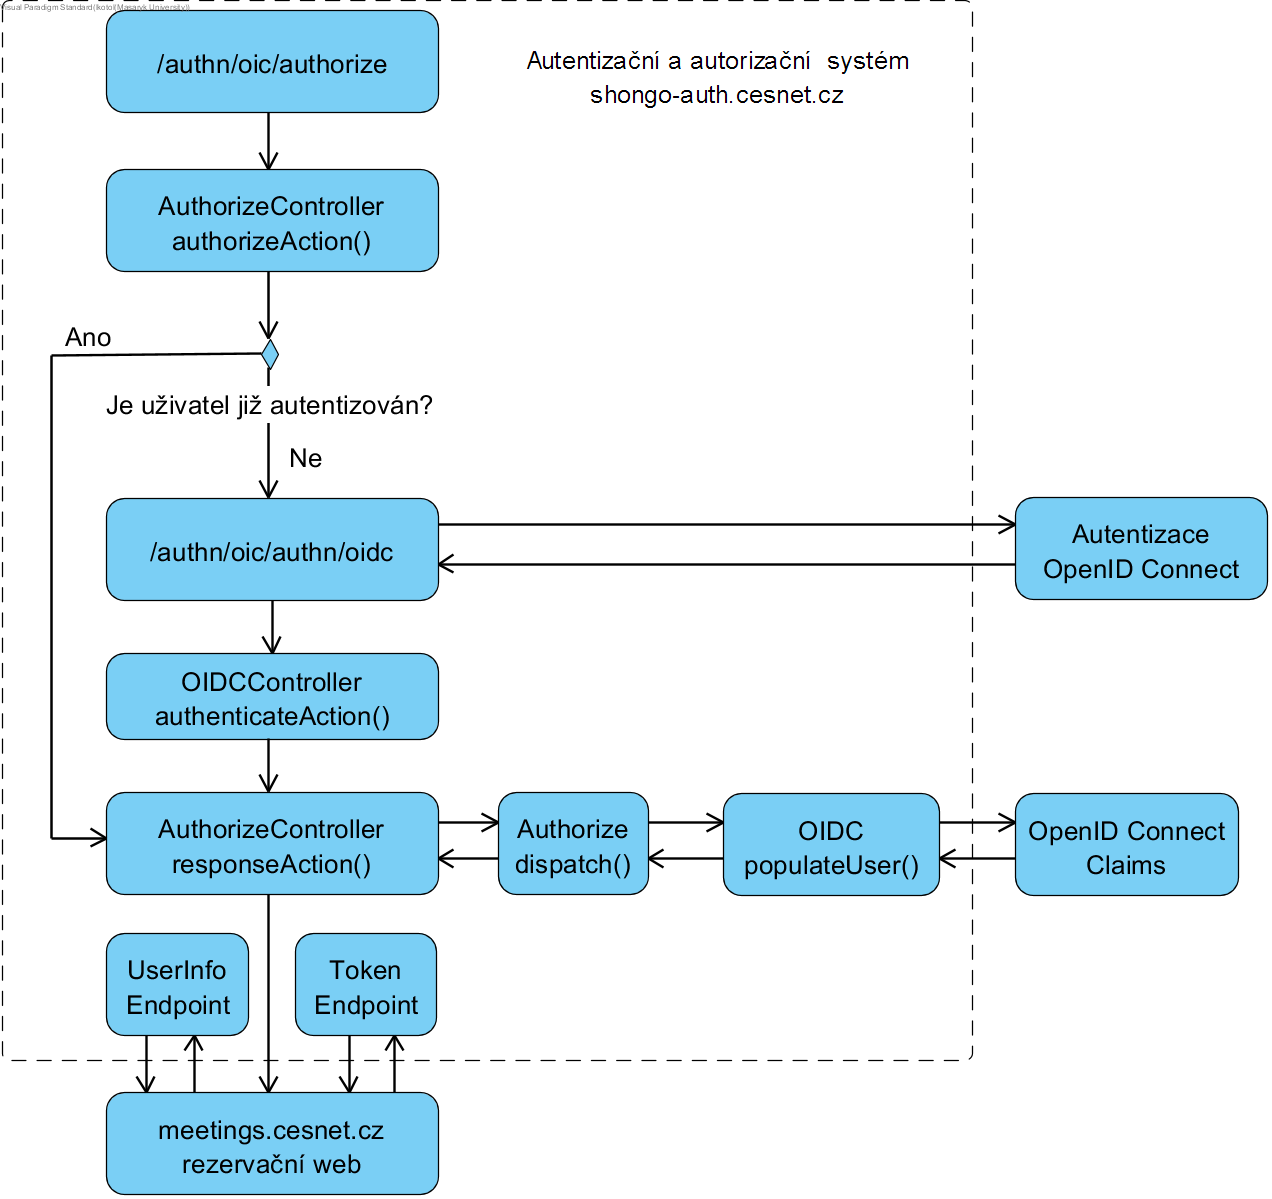
\includegraphics[width=12.8cm]{pics/shongo-auth-layer-new} 
\label{fig:shongoAuthnProcessNew}
\end{figure}


\subsection{Implementace autorizační logiky na serveru shongo-auth.cesnet.cz}
\label{ShongoImpl-authr}    
V této kapitole představuji kroky, které jsem provedl v rámci implementace vrstvy zajišťující prosazování autorizační politiky. Jde o autorizační politiku, ve které bylo nutné zajistit kontrolu příslušnosti uživatele do skupiny einfra. Přítomnost uživatele ve skupině einfra zaručuje tzv. \textbf{LoA} úrovně dva. Jak již bylo uvedeno výše, \textbf{LoA (Level of Assurance)} je úroveň záruky vyjadřující míru spolehlivosti prostředků pro elektronickou identifikaci při určování totožnosti dané osoby. Opět v tomto kontextu \textbf{LoA} úrovně dva značí, že uživatel je schopný ověřit svoji identitu pomocí přihlašovacího hesla. Jde tedy o bezpečnostní záruku autorizační vrstvě systému \path{shongo-auth.cesnet.cz}, že se jedná řádně přihlášeného uživatele. Ve stávající implementaci byly informace o příslušnosti uživatele do skupiny einfra zjišťována pomocí volání webové služby Perun. Jelikož nynější autorizační vrstva nevyužívá již volání webové služby Perun, musel být způsob představené kontroly příslušnosti uživatele do skupiny einfra nahrazen. 

\par

V rámci implementace představené autorizace jsem vytvořil validátor \path{OIDCUser.php}. Úkolem vytvořeného validátoru \path{OIDCUser.php} je kontrola, zda autentizovaný uživatel patří do skupiny einfra. Logika zmíněného validátoru je založena na algoritmu, který ověřuje zda je v seznamu skupin \textbf{OIDC\_CLAIM\_eduPersonEntitlement} do kterých uživatel patří přítomen řetězec \path{urn:geant:cesnet.cz:group:einfra:einfra\#perun.cesnet.cz}. Uvedený řetězec reprezentuje zmiňovanou skupinu einfra. Pokud uživatel do požadované skupiny patří, je oprávněn využívat služeb portálu \path{meetings.cesnet.cz}. Tedy běh algoritmu pokračuje stejným způsobem jako v stávající implementaci, který popisuji v kapitole \hyperref[meetings-old]{2.1.2}. Pokud uživatel do skupiny einfra nepatří, je přesměrován na stránku Proxy IdP infrastruktury CESNET s registrací. Zde uživatel odsouhlasí přiřazení do skupiny einfra. Dále jsou v obou případech nastaveny objektu představujícího uživatele dodatečné autentizační informace. Na základě těchto autentizačních informací je po přesměrování do systému \path{meetings.cesnet.cz} uživateli umožněno vytvářet rezervační požadavky. Jde o identifikátor autorizačního serveru, časová značka představující čas autentizace a pevně danou hodnotu \textbf{LoA} úrovně dva. Je vhodné připomenout, že jestliže je uživatel členem skupiny einfra, potom je mu garantováno \textbf{LoA} úrovně dva. Dále je běh algoritmu obdobný jako ve stávající implementaci a prohlížeč je tedy nakonec s vygenerovaným autorizačním kódem přesměrován na úvodní stránku přihlášeného uživatele systému \path{meetings.cesnet.cz}.

\par




Na závěr této kapitoly je důležité zmínit, že v rámci implementace byla zkopírována celá autentizační a autorizační vrstva portálu \path{meetings.cesnet.cz} do adresáře \path{/app/shongo-authn/}. Přístup k uvedenému adresáři přes webový server Apache je nastaven v konfiguračním souboru \path{/etc/apache2/sites-available/default-ssl} pomocí URL adresy \path{shongo-auth.cesnet.cz/oidc-authn}. Uvedená URL adresa je chráněna OpenID Connect modulem Apache, který byl nakonfigurován v kapitole \hyperref[sec:mod-conf]{4.1.3}.

\subsection{Odstranění závislosti datové vrstvy systému meetings.cesnet.cz na webové službě Perun}
\label{zpracovaniAUlozeniPerun}
V následujících odstavcích se zabývám popisem procesu odstranění závislosti datové vrstvy systému meetings.cesnet.cz na webové službě Perun. Je vhodné poznamenat, že ve stávající implementaci datové vrstvy systému \path{meetings.cesnet.cz} se webová služba Perun používala k získání dodatečných uživatelských údajů. Jde o uživatelské údaje, které autentizační modul Shibboleth neposkytoval a proto bylo nutné k jejich získání využívat webovou službu Perun. K jakékoliv práci s uživatelem tedy bylo vždy nutné volat webovou službu Perun, jelikož tyto informace nebyli ukládány do databáze. 

\par 

Jak je patrné z návrhu nové autentizační a autorizační vrstvy systému \path{meetings.cesnet.cz}, který se nachází v kapitole \hyperref[shong-proposal]{2.3.2}, v nové implementaci se již webová služba Perun z důvodu zvýšení dostupnosti nepoužívá. Abychom zachovali dostupnost nezbytných uživatelských informací, muselo dojít k jednorázovému zpracování a uložení těchto uživatelských dat do databáze. K získaní zmiňovaných uživatelských údajů byla jednorázově využita právě data z webové služby Perun. Před samotným popisem zpracování a uložení uživatelských dat získaných z webové služby Perun je vhodné připomenout následující výrazy, které jednoznačně identifikují uživatele. První z nich je identifikátor \textbf{perun id}, který jednoznačně identifikuje uživatele v rámci webové služby Perun. Další identifikátor, tzv. \textbf{einfra id} identifikuje uživatele v rámci Proxy IdP infrastruktury provozované sdružením CESNET. Je důležité poznamenat, že autorizační server OpenID Connect neumožňuje získat uživatelský identifikátor \textbf{perun id} prostřednictvím \textbf{Claims}. Protože systém \path{meetings.cesnet.cz} tento identifikátor \textbf{perun id} využívá jako primární klíč uživatele v rámci webové služby Perun byla nutná náhrada zmíněného identifikátoru za \textbf{einfra id}. Dalším důvodem náhrady identifikátoru \textbf{perun id} za \textbf{einfra id} bylo zachování vztahu mezi autentizovaným uživatelem a jeho aplikačními daty v systému \path{meetings.cesnet.cz}. V následujících odstavcích popisuji dílčí kroky které jsem provedl v rámci představeného jednorázového zpracování a uložení uživatelských dat získaných z webové služby Perun. 

\par

Jak již bylo nastíněno, první fáze implementace tvořila nahrazení identifikátoru \textbf{perun id} za \textbf{einfra id}. Uvedený identifikátor se nachází v tabulkách \textbf{person}, \textbf{user\_settings}, \textbf{resource}, \textbf{acl\_identity}, \textbf{reservation} a \textbf{abstract\_reservation\_request}. V rámci představené modifikace datové vrstvy byly do tabulek \textbf{person} a \textbf{user\_settings} doplněny i dodatečné údaje o uživateli. Jde o údaje o uživatelově jménu, emailové adrese, organizaci, preferovaném jazyku a časové zóně, které byly dříve získávány pomocí webové služby Perun. Představené uživatelské údaje se ve stávající implementaci získávaly dynamicky až ve chvíli, kdy bylo potřeba manipulovat s uživatelem. Webová služba Perun se v nové implementaci již nepoužívá a proto musely být uživatelské údaje opatřeny jiným způsobem. K získání údajů o aktuálně autentizovaném uživateli posloužil nainstalovaný Apache modul umožňující získat \textbf{Claims} z autorizačního serveru OpenID Connect. Implementaci získání a zpracování údajů o aktuálně autentizovaném uživateli popisuji v kapitole \hyperref[ShongoImpl-authn]{4.3.1}. Pro všechny stávající uživatele v systému \path{meetings.cesnet.cz} musely být jejich uživatelské údaje uloženy do databáze. Výhodou je, že tabulky obsahují požadované sloupce, protože se s zmíněnými uživatelskými údaji již pracovalo při správě tzv. anonymních uživatelů, což jsou uživatelé, kteří nepatří do skupiny einfra. 
\par

Algoritmus, který popisované jednorázové zpracování uživatelských údajů z webové služby Perun provedl jsem implementoval v jazyce Java. Zmíněný algoritmus obsahuje následující kroky pro každou z tabulek \textbf{person}, \textbf{user\_settings}, \textbf{resource}, \textbf{acl\_identity}, \textbf{reservation} a \textbf{abstract\_reservation\_request}. Počáteční fází bylo získání všech záznamů s uživatelskými identifikátory \textbf{perun id} z dotyčné tabulky. V dalším kroku byl pro každý záznam s identifikátorem \textbf{perun id} vytvořen GET požadavek na rozhraní webové služby Perun, které je přítomno na URL adrese \path{https://shongo-auth.cesnet.cz/perun/users/\{perun id\}}. Uvedený dotaz na API webové služby Perun vrátí požadované informace o uživateli ve formátu JSON jehož strukturu popisuji v příloze \hyperref[table:perunws:user]{A.1}.

\par

Dalším krokem algoritmu bylo získání identifikátoru \textbf{einfra id} z představené odpovědi. Tento identifikátor se nachází v poli \textbf{sources}, představující poskytovatele identit, konkrétně v atributu \textbf{sources.login}. Jelikož nás zajímá pouze identifikátor v rámci Proxy IdP infrastruktury CESNET, musel algoritmus najít poskytovatele identit, který má v atributu \textbf{sources.name} řetězec \textbf{https://login.cesnet.cz/idp/}. Jestli algoritmus našel zmíněného poskytovatele identit, v atributu \textbf{sources.login} se nachází \textbf{perun id} hledaného uživatele. Tento údaj byl poznamenán do nově vytvořeného objektu, představujícího uživatele. Do toho objektu byly dále uloženy informace o uživatelově jménu, emailové adrese, organizaci, preferovaném jazyku a časové zóně. 

\par

V závěrečné fázi algoritmu je pro každého takto vytvořeného objektu uživatele v aktuálně zpracovávané tabulce nahrazeno \textbf{perun id} za \textbf{einfra id}. Jak již bylo zmíněno, speciálním případem jsou tabulky \textbf{person} a \textbf{user\_settings}, kde došlo navíc k vložení chybějících uživatelských údajů. Následující obrázek 4.1 ilustruje schéma tabulek \textbf{person} a \textbf{user\_settings}. 

\begin{figure}[H]
\label{fig:erd-person-user-settings}
\caption{Struktura tabulek \textbf{person} a \textbf{user\_settings}}
\centering
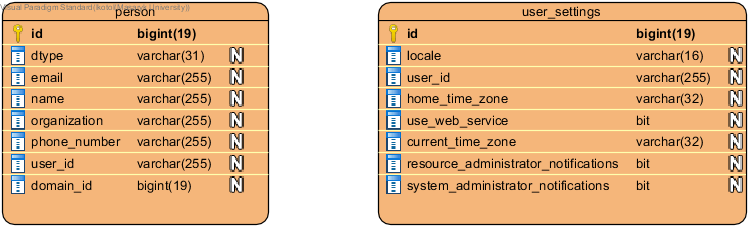
\includegraphics[width=12.8cm]{pics/erd-person-user_settings} 
\end{figure}
\par 

Zmíněnou modifikaci tabulky \textbf{person} pro každého uživatele ilustruje následující SQL dotaz.

\begin{lstlisting}[
           language=SQL,
           showspaces=false,
           basicstyle=\footnotesize\ttfamily,
           commentstyle=\color{gray},
           backgroundcolor=\color{background},
           frame=lines
        ]
UPDATE person SET 
user_id = {einfra_id},
email = {email},
name = {name},
organization = {organization},
WHERE id = {id};
\end{lstlisting}

Obdobně při modifikaci tabulky \textbf{user\_settings} byl použit následující SQL dotaz. 

\begin{lstlisting}[
           language=SQL,
           showspaces=false,
           basicstyle=\footnotesize\ttfamily,
           commentstyle=\color{gray},
           backgroundcolor=\color{background},
           frame=lines
        ]
UPDATE user_settings SET 
user_id = {einfra_id},
home_time_zone = {time_zone},
current_time_zone = {current_time_zone},
locale = {locale},
WHERE id = {id};
\end{lstlisting}

Pomocí spuštění uvedených dotazů, byly uloženy uživatelské údaje pro každého uživatele do tabulek \textbf{person} a \textbf{user\_settings}. Dále již stačilo vhodným způsobem modifikovat rezervační systém \path{meetings.cesnet.cz} k tomu, aby využíval uložená uživatelská data místo volání webové službě Perun. Zmíněnou adaptaci logické vrstvy systému \path{meetings.cesnet.cz} na provedené změny v rámci implementace nové autentizační a autorizační vrstvy popisuji v kapitole \hyperref[ShongoImpl-web]{4.3.4}. 

\par

Je důležité poznamenat, že popsané náhradě identifikátorů předcházela modifikace databázového schématu, protože nový identifikátor \textbf{einfra id} by překračoval maximální povolenou délku sloupce vyhrazenou pro \textbf{perun id}. Uvedený sloupec s uživatelským identifikátorem se používal v tabulkách \textbf{person}, \textbf{user\_settings}, \textbf{resource}, \textbf{acl\_identity}, \textbf{reservation} a \textbf{abstract\_reservation\_request}. Jelikož je databázové schéma definované pomocí technologie Hibernate, došlo ke změně délky sloupce jak na straně databáze, tak na straně třídy definující vlastnosti používaných tabulek. 

\par  

Na straně systému \path{meetings.cesnet.cz} jsem provedl změnu délky sloupce v souboru \path{cz/cesnet/shongo/controller/api/Controller.java}. Uvedená změna se týkala proměnné \path{USER_ID_COLUMN_LENGTH}, která definuje délku sloupce. Sloupec je typu VARCHAR a byl změněn z délky 32 na 255. Dále byla provedena změna délky sloupce v databázových tabulkách pomocí následujícího SQL příkazu.

\begin{lstlisting}[
           language=SQL,
           showspaces=false,
           basicstyle=\footnotesize\ttfamily,
           commentstyle=\color{gray},
           backgroundcolor=\color{background},
           frame=lines
        ]
ALTER TABLE {nazev_tabulky}  
ALTER COLUMN {nazev_sloupce}
TYPE VARCHAR (255);
\end{lstlisting}

\par

Další krok který vedl k odstranění závislosti na webové službě Perun tvořilo uložení dat určených pro autorizaci. Jde o data, která se ve stávající implementaci získávala prostřednictvím webové služby Perun. Jak již bylo poznamenáno, v nynější implementaci se webová služba Perun nepoužívá a proto muselo dojít k uložení požadovaných dat. Je důležité poznamenat, že při vytváření speciálních rezervačních požadavků se v systému \path{meetings.cesnet.cz} kontroluje, zda je uživatel oprávněn tyto operace provádět. Jde o specifické zdroje, určené pro uživatele v konkrétních skupinách. Zmíněná kontrola oprávnění vytvářet požadavky na specifické zdroje se realizuje vůči příslušnosti uživatele do skupin s následujícími URN. 
\begin{itemize}
    \item urn:geant:cesnet.cz:group:einfra:projects:shongo:users:\linebreak cesnet\#perun.cesnet.cz
    \item urn:geant:cesnet.cz:group:einfra:projects:shongo:users:\linebreak ufe\#perun.cesnet.cz
    \item urn:geant:cesnet.cz:group:einfra:projects:shongo:users:\linebreak uvt\#perun.cesnet.cz
    \item urn:geant:cesnet.cz:group:einfra:projects:shongo:system:\linebreak admins\#perun.cesnet.cz
    \item urn:geant:cesnet.cz:group:einfra:projects:shongo:users:\linebreak shongo\#perun.cesnet.cz
\end{itemize}

Ve stávající implementaci byla uvedená kontrola uskutečňována prostřednictvím webové služby Perun. Voláním webové služby Perun si systém \path{meetings.cesnet.cz} získal skupiny, do kterých uživatel patří. Konkrétně šlo o identifikátor dané skupiny, tzv. \textbf{group id}. Kontrola, zda je umožněno uživatelovi rezervovat specifické zdroje potom probíhala vůči získaným \textbf{group id} skupin z webové služby Perun, jejichž \textbf{group id} se nachází v databázi systému \path{meeting.cesnet.cz}. Na základě této informace bylo dále umožněno rezervovat kapacity ve vybraných místností. Jelikož nová implementace autentizační a autorizační vrstvy systému \path{meetings.cesnet.cz} již není závislá na webové službě Perun, musela být prováděná kontrola nahrazena jiným mechanizmem. 

\par
První část modifikace představené kontroly skupin uživatele sestávala z nahrazení \textbf{group id} všech skupin uložených v databázi systému \path{meetings.cesnet.cz} za URN \cite{rfc2141} dotyčné skupiny. Uvedené URN (Uniform Resource Name) je textový řetězec, který se používá k jednoznačné identifikaci obecného zdroje. Důvodem nahrazení identifikátoru skupiny za URN je fakt, že infrastruktura Proxy IdP sdružení CESNET v \textbf{Claims} neposkytuje \textbf{group id}, ale pouze URN skupin, kterých je uživatel členem. 

\par 

Tabulka, které se týká zmiňované nahrazení identifikátoru \textbf{group id} za URN se nazývá \textbf{acl\_identity}. Uvedená tabulka má sloupce \textbf{id}, \textbf{principal\_id} a \textbf{type} ve kterých si drží své záznamy. Údaj ve sloupci \textbf{type} může nabývat hodnoty \textbf{USER} nebo \textbf{GROUP}. Jestliže nabývá hodnoty \textbf{USER}, potom je ve sloupci \textbf{principal\_id} obsažen identifikátor uživatele \textbf{perun id}. Pokud sloupec \textbf{type} obsahuje hodnotu \textbf{GROUP}, potom se ve sloupci \textbf{principal\_id} nachází identifikátor skupiny. Tato informace musela být zohledněna při nahrazování identifikátoru \textbf{principal\_id}. 

\par 
Pokud hodnota ve sloupci \textbf{principal\_id} představovala \textbf{perun id}, postupoval algoritmus jako v předchozím popisovaném případě a byl nahrazen za \textbf{einfra id}. Jestliže hodnota ve sloupci \textbf{principal\_id} představovala identifikátor skupiny, tento identifikátor musel být nahrazen za URN  dotyčné skupiny. Zmíněné nahrazení za URN bylo provedeno jednorázově pomocí webové služby Perun. Tentokrát již ale s použitím API rozhraní k získání dodatečných informací o požadované skupině. Volání představeného rozhraní bylo provedeno pomocí GET požadavku na URL adresu  \path{https://shongo-auth.cesnet.cz/perun/groups/\{group id\}}. Uvedený GET požadavek vrátil data o skupině v JSON struktuře. Zmíněnou JSON strukturu popisuji v příloze \hyperref[table:perunws:group]{A.2}.
\par
Z uvedené odpovědi ve formátu JSON byl použit atribut \linebreak\textbf{unique\_name}, který reprezentuje požadované URN skupiny. Za tuto hodnotu URN skupiny byla potom hodnota v sloupci \textbf{principal\_id} pomocí SQL příkazu nahrazena. Popsaný postup byl zopakován pro každý záznam v tabulce \textbf{acl\_identity}, kde hodnota ve sloupci \textbf{principal\_id} představovala identifikátor skupiny \textbf{group id}. 
\par 

Popsaná procedura vedla k uložení URN skupiny do tabulky \textbf{acl\_identity}. Aby odstranění volání webové služby Perun bylo kompletní, musela být provedena implementační změna, která adaptuje systém \path{meetings.cesnet.cz} na provedené úpravy v databázi. Jedná se o odstranění závislosti na volání webové služby Perun, která poskytovala informace o skupinách uživatele. Takto získané identifikátory skupin se dříve kontrolovaly vůči \textbf{group id} v tabulce \textbf{acl\_identity}. Implementace OpenID Connect provozovaná v rámci Proxy IdP infrastruktury CESNETu ale poskytuje pouze URN skupin, do kterých uživatel patří. Na tuto skutečnost musela být kontrola příslušnosti uživatele adaptována. Implementaci zmíněné adaptace na straně systému \path{meetings.cesnet.cz} na nahrazení \textbf{group id} za URN skupiny a další úpravy popisuji v kapitole \hyperref[ShongoImpl-web]{4.3.4}. 

\subsection{Adaptace logické vrstvy systému meetings.cesnet.cz}
\label{ShongoImpl-web}
V této sekci se věnuji tématu, jakým způsobem musela být logická vrstva rezervačního systému \path{meetings.cesnet.cz} adaptována na provedené změny v rámci implementace nové autentizační a autorizační vrstvy. 
\par

Hlavní fází adaptace logické vrstvy systému \path{meetings.cesnet.cz} na nově vytvořenou autentizační a autorizační strukturu byla eliminace využívání webové služby Perun. Jak již bylo výše uvedeno, webová služba Perun se v systému \path{meetings.cesnet.cz} využívala k získání dodatečných informací o uživatelích a skupinách. Zmíněné uživatelské informace se získávaly dynamicky. V rámci této diplomové práce jsem zmíněné dodatečné informace o uživateli a skupině uložil do databáze a tudíž nyní není nutné všechny uložené údaje získávat voláním pomocí webové služby Perun. Popisu odstranění závislosti na webové službě Perun, jednorázového uložení uživatelských údajů a informacích o skupinách se věnuji v kapitole \hyperref[zpracovaniAUlozeniPerun]{4.3.3}. Jelikož se uživatelské informace po zmíněné upravě datové vrstvy systému \path{meetings.cesnet.cz} nacházejí v databázi, můžeme tyto informace nyní získat právě s využitím databázového systému. V následujících odstavcích popisuji konkrétní mechanizmus, jakým způsobem jsem upravil metody, tak aby místo webové služby Perun využívaly datovou vrstvu systému \path{meetings.cesnet.cz}. 

\par
Před samotným popisem adaptace logické vrstvy rezervačního systému \path{meetings.cesnet.cz} je vhodné znovu připomenout význam identifikátorů \textbf{perun id} a \textbf{einfra id}. Identifikátor \textbf{perun id} jednoznačně určuje uživatele v rámci webové služby Perun. Druhý identifikátor \textbf{einfra id}, jednoznačně identifikuje uživatele v Proxy IdP infrastruktuře CESNETu. 
\par V rámci adaptace logické vrstvy systému \path{meetings.cesnet.cz} na provedené změny jsem modifikoval chování třídy \path{cz.cesnet.shongo.controller.authorization.ServerAuthorization}. Konkrétně šlo o modifikaci metod sloužících k získání uživatelských informací pomocí \textbf{perun id} (\path{onGetUserDataByUserId}), získání uživatelského \textbf{perun id} pomocí \textbf{eduPersonPrincipalName} (\path{onGetUserIdByPrincipalName}),\linebreak získání skupiny pomocí \textbf{group id} (\path{onGetGroup}) a získání skupin kterých je uživatel členem (\path{onListUserGroupIds}). 


\subsubsection{Metoda \texttt{onGetUserDataByUserId}}

Jak již bylo poznamenáno, první z metod \path{onGetUserDataByUserId} je v systému \path{meetings.cesnet.cz} využívána k získání informací o konkrétním uživateli pomocí jeho identifikátoru. Ve stávající implementaci se jako referenční identifikátor využívalo pouze \textbf{perun id}. V nové implementaci se uživatelské informace vyhledávají i pomocí identifikátoru \textbf{einfra id}. Funkcionalitu vyhledávání uživatele prostřednictvím \textbf{perun id} pomocí webové služby Perun jsem ponechal, protože je využívána při přidávání dalších účastníku ve vytvářeném rezervačním požadavku. 

\par 

Jak jsem v této kapitole již uvedl, prostřednictvím metody \linebreak \path{onGetUserDataByUserId} je nově umožněno vyhledávat uživatele i pomocí identifikátoru \textbf{einfra id}. Zmíněné vyhledávání uživatelů pomocí \textbf{einfra id} je realizováno oproti uloženým uživatelským údajům v databázi systému \path{meetings.cesnet.cz}. Konkrétně jde o tabulky \textbf{person} a \textbf{user\_settings} v kterých se uživatelské údaje vyhledávají. Uvedené vyhledávání s použitím identifikátoru \textbf{einfra id}, je nyní možné, protože byla provedena transformace uživatelských identifikátorů všech stávajících uživatelů v tabulkách systému \path{meetings.cesnet.cz} z \textbf{perun id} na \textbf{einfra id}. Dále také došlo k uložení dodatečných informací o uživateli, které se dříve získávaly pomocí webové služby Perun. Představené jednorázové uložení dodatečných uživatelských informací je popsáno v kapitole \hyperref[zpracovaniAUlozeniPerun]{4.3.3}. 

\subsubsection{Metoda \texttt{onGetUserIdByPrincipalName}}

Další modifikovaná metoda, jejíž chování jsem adaptoval na provedené změny v autentizační a autorizační vrstvě systému \path{meetings.cesnet.cz} se nazývá \path{onGetUserIdByPrincipalName}. Uvedená metoda dříve sloužila k získání identifikátoru \textbf{perun id} na základě poskytnutého \textbf{eduPersonPrincipalName} uživatele prostřednictvím webové služby Perun. Zmíněné \textbf{eduPersonPrincipalName} je jednoznačný identifikátor v rámci federace, mající formát uživatelské\_jméno@doména. V nové implementaci je nyní místo \textbf{perun id} vyhledáváno \textbf{einfra id}. Zmíněné \textbf{einfra id} je vyhledáváno v databázi systému \path{meetings.cesnet.cz}, konkrétně vůči všem uživatelským záznamům v tabulce \textbf{person}. Jak již bylo zmíněno, vyhledávání uživatelských údajů v databázi je v nynější implementaci umožněno díky předcházejícímu uložení dodatečných uživatelských údajů do tabulek \textbf{person} a \textbf{user\_settings}.

\subsubsection{Metoda \texttt{onGetGroup}}

Další fáze adaptace na odstranění závislosti webové služby Perun sestávala z modifikace metody \textbf{onGetGroup}. Uvedená metoda \textbf{onGetGroup} slouží získání k údajů o skupině na základě identifikátoru dané skupiny. Ve stávající implementaci metoda obdobně jako v předchozích případech využívala volání webové služby Perun. V nynější implementaci je chování představené metody koncipováno odlišným způsobem. Logiku uvažované metody \textbf{onGetGroup} jsem pozměnil tak, aby místo volání webové služby Perun, využívala uložené údaje v databázi. Konkrétně jde o tabulku \textbf{acl\_identity} v které se nyní údaje o skupinách vyhledávají. 

\subsubsection{Metoda \texttt{onListUserGroupIds}}
Poslední modifikovaná metoda v třídě \path{cz.cesnet.shongo.controller.authorization.ServerAuthorization} se nazývá \textbf{onListUserGroupIds}. Funkcionalita představené metody ve stávající implementaci spočívala v nalezení všech \textbf{group id} skupin, kterých je uživatel s příslušným \textbf{perun id} členem. Je důležité zmínit, že metoda \textbf{onListUserGroupIds} se využívá ke kontrole příslušnosti uživatele do skupin, jejichž členové mají povoleno rezervovat speciální zdroje. Uvažovaná kontrola probíhala vůči uloženým záznamům s příslušnými \textbf{group id} v databázové tabulce \textbf{acl\_identity} systému \path{meetings.cesnet.cz}. Na základě příslušných \textbf{group id} uložených v tabulce \textbf{acl\_identity} bylo potom uživateli umožněno alokovat speciální zdroje. Jelikož došlo k transformaci \textbf{group id} na identifikátor skupiny URN ve zmiňované tabulce \textbf{acl\_identity}, musel být algoritmus metody \textbf{onListUserGroupIds} na tyto změny adaptován. Uvedenému nahrazení jednorázovému identifikátoru \textbf{group id} za URN skupin v tabulce \textbf{acl\_identity} se věnuji v kapitole \hyperref[zpracovaniAUlozeniPerun]{4.3.3}. 

\par

Algoritmus představené metody \textbf{onListUserGroupIds} jsem modifikoval tak, aby místo seznamu identifikátorů skupin \textbf{group id} vracel seznam URN dotyčných skupin. Uvedené funkcionality bylo dosaženo prostřednictvím \textbf{UserInfo Endpointu}, který jsem upravil tak, aby vracel seznam URN skupin v kterých je přihlášený uživatel členem. Aby metoda \textbf{onListUserGroupIds} mohla využívat \textbf{UserInfo Endpoint}, musel být nahrazen vstupní argument metody \textbf{perun id} za \textbf{Access Token}. Je důležité poznamenat, že nyní lze tedy získat pouze takové URN skupin, jejichž je aktuálně přihlášený uživatel členem. Tato funkcionalita je dostačující, protože v rámci rezervačního procesu se kontrolují práva na rezervace speciálních zdrojů pouze přihlášeným uživatelům. Díky této modifikaci mohou být získané URN skupin spárována s uloženými URN skupin v databázi. Následně tedy může dojít ke kontrole zda, je aktuálně přihlášenému uživateli dovoleno využívat specifické zdroje, podmíněné příslušností uživatele do určitých skupin.

\par

Jak bylo výše popsáno, všechny zmíněné volání webové služby Perun byly vhodným způsobem nahrazeny a zachovala se tedy plná funkcionalita systému \path{meeting.cesnet.cz}.

\subsubsection{Ostatní změny provedené v rámci adaptace}
Další fází adaptace na provedené změny v autentizační a autorizační vrstvě byla změna URL adresy výchozího bodu autentizace, \textbf{UserInfo endpointu} a \textbf{Token endpointu}. Zmíněné URL adresy, na které je nově rezerevační systém \path{meetings.cesnet.cz} napojen jsou popsány v příloze \hyperref[oidcEndpoints]{B}. Důvodem představené změny bylo aby zdroje, jejichž využití vyžaduje autentizaci pomocí protokolu OpenID Connect, odpovídaly nastavení definovaném v rámci konfigurace Apache. \par


Výchozí část URL adresy, která slouží jako prefix URL adresy zajištující autentizaci a autorizaci je definována v souboru \path{cz/cesnet/shongo/client/web/ClientWebConfiguration.java}. Zmíněnou hodnotu, která je v stávající implementaci nastavena na URL adresu \path{/authn/oic} vrací metoda \path{getAuthenticationServerUrl}. Představenou část URL adresy jsem pozměnil na hodnotu \path{/oidc-authn/oic}, tak aby odpovídala URL adresám, které jsou chráněny OpenID Connect autentizací. Ostatní parametry URL adresy nebyly změněny. 
\par

V poslední řadě jsem v rámci implementace této diplomové práce vytvořil logiku, která na straně systému \path{meetings.cesnet.cz} zajišťuje, že se při vytváření rezervačních požadavků uloží všechny potřebné informace o aktuálním přihlášeném uživateli. Ve stávající implementaci byl tento proces odlišný. Po vytvoření rezervačního požadavku se pouze uložil identifikátor uživatele \textbf{perun id}. Následným voláním webové služby Perun se potom získávaly dodatečné údaje o uživateli. V nynější implementaci jsou uloženy všechny informace o aktuálně přihlášeném uživateli a tudíž není potřeba využívat webovou službu Perun. 

\chapter{Závěr}
Cílem diplomové práce bylo vytvořit novou autentizační a autorizační infrastrukturu pro stávající video a webkonferenční prostředí provozované sdružením CESNET. V rámci vypracování této diplomové práce byla provedena analýza stávající autentizační a autorizační infrastruktury. Dále byl vyhotoven návrh a následná úspěšná implementace nové autentizační a autorizační infrastruktury.  

\par 

Konkrétně se jednalo o vytvoření nové autentizační a autorizační vrstvy pro systémy Adobe Connect a \path{meetings.cesnet.cz}. Jedním z klíčových požadavků bylo, aby autentizační a autorizační vrstva uvedené video a webkonferenční platformy byla integrováa do stávající Proxy IdP infrastruktury pomocí technologie OpenID Connect. Všechny představené cíle byly splněny a jsou dokumentovány v předcházejících kapitolách. 

\par
Implementovaná autentizační a autorizační vrstva nově není závislá na webové službě Perun. Přínosem uvedené změny je fakt, že webová služba Perun vykazovala při svém provozu známky nedostupnosti a nová implementace tedy zvyšuje robustnost celého video a webkonferenčního prostředí. Neméně důležitým faktem, který přispívá k lepší udržitelnosti celé autentizační a autorizační infrastruktury, je že při eliminaci závislosti na webové službě Perun došlo k výraznému zjednodušení zmíněné infrastruktury. Dalším přínosem nově vytvořené autentizační a autorizační infrastruktury je možnost připojit se do video a webkonferenčního prostředí pomocí identit z mezinárodní akademické federace eduGAIN. V neposlední řadě, napojením na novou autentizační a autorizační infrastrukturu vznikla možnost využívat dalších neakademických poskytovatelů identit jako jsou společnosti Google, Facebook, LinkedIn a Github. 

\par

Je vhodné zmínit, že nově vytvořená autentizační a autorizační vrstva systému \path{meetings.cesnet.cz} je stále otevřená k dalšímu zdokonalení. Netriviálním zjednodušením autentizační a autorizační vrstvy by mohlo být odstranění autorizačního serveru \path{shongo-auth.cesnet.cz}. Uvedený server slouží jako vrstva mezi autorizačním serverem v Proxy IdP infrastruktuře provozované sdružením CESNET a samotným rezervačním systémem \path{meetings.cesnet.cz}. V rámci snížení komplexnosti autentizační a autorizační vrstvy systému \path{meetings.cesnet.cz} se tedy nabízí tuto mezi vrstvu odstranit. Jelikož je server \path{shongo-auth.cesnet.cz} mimo jiné zodpovědný za autorizaci uživatelů, představená funkcionalita by musela být přesunuta až na stranu systému \path{meetings.cesnet.cz}. 

\par 

Celkově hodnotím přínos této diplomové práce kladně, jelikož značným způsobem zdokonalila mé znalosti v oblasti autentizačních a autorizačních systémů.

\printbibliography[title={Literatura}]

\appendix %% Start the appendices.


\chapter{Struktura odpovědí HTTP požadavků webové služby Perun}

\section{Získání uživatele}
\label{table:perunws:user}
Následující příklad ilustruje získané údaje o uživateli pomocí HTTP GET požadavku na URL adresu \path{https://shongo-auth.cesnet.cz/perun/users/{perun id}}.

\begin{lstlisting}[language=json,firstnumber=1]
{
    "id": 57025,
    "first_name": "Lukas",
    "last_name": "Kotol",
    "principal_names": [
        "3e21c29ec2b940c3336b80c5141de4e79ba82f36@einfra.cesnet.cz"
    ],
    "timezone": "Europe/Prague",
    "language": "cs",
    "organization": "Masarykova univerzita",
    "mail": "433265@mail.muni.cz",
    "display_name": "Lukas Kotol",
    "sources": [
        {
            "id": 149552,
            "name": "https://login.cesnet.cz/idp/",
            "loa": 0,
            "login": "3e21c29ec2b940c3336b80c5141de4e79ba82f36@einfra.cesnet.cz"
        }
    ],
    "member_id": 70076,
    "member_status": "VALID",
    "_links": {
        "self": {
            "href": "https://shongo-auth.cesnet.cz/perun/users/57025"
        }
    }
}
\end{lstlisting}
V následující tabulce je uveden význam získaných atributů v předešlé odpovědi.
\begin{table}[H]
\begin{tabular}{|l|l|}
\hline
\path{id (int)}                   & \parbox[t]{6.3cm}{identifikátor uživatele v rámci webové Perun služby } \\ \hline
\path{first_name (String)}       & křestní jméno uživatele \\ \hline
\path{last_name (String)}        & příjmení uživatele \\ \hline
\path{principal_names (Array)}   & \parbox[t]{6.3cm}{pole obsahující všechny eduPersonPrincipalName uživatele} \\ \hline
\path{language (String)}          & preferovaný jazyk uživatele \\ \hline
\path{organization (String)}      & výchozí organizace uživatele \\ \hline
\path{phone (String)}             & telefonní číslo uživatele \\ \hline
\path{mail (String)}              & emailová adresa uživatele \\ \hline
\path{display_name (String)}     & úplné jméno uživatele \\ \hline
\path{sources (Array)}            & \parbox[t]{6.3cm}{pole poskytovatelů identit, v kterých je uživatel registrován} \\ \hline
\path{sources.id (int)}           & \parbox[t]{6.3cm}{identifikátor poskytovatele identit} \\ \hline
\path{sources.name (String)}      & název poskytovatele identit \\ \hline
\path{sources.loa (int)}          & \parbox[t]{6.3cm}{úroveň zabezpečení poskytovatele identit}  \\ \hline
\path{sources.login (String)}     & \parbox[t]{6.3cm}{identifikátor uživatele u daného poskytovatele identit} \\ \hline
\path{member_id (int)}           & \parbox[t]{6.3cm}{identifikátor ve virtuální organizaci \path{meetings.cesnet.cz}} \\ \hline
\path{member_status (String)}    & informace o stavu uživatele \\ \hline
\path{_links.self.href (String)} & \parbox[t]{6.3cm}{URL adresa aktuálního HTTP GET požadavku} \\ \hline
\end{tabular}
\end{table}

\section{Získání skupiny}
\label{table:perunws:group}

Následující příklad ilustruje získané údaje o skupině pomocí HTTP GET požadavku na URL adresu \path{https://shongo-auth.cesnet.cz/perun/groups/{group id}}.

\begin{lstlisting}[language=json,firstnumber=1]
{
    "id": 9804,
    "name": "uvt",
    "unique_name": "projects:shongo:users:uvt",
    "type": "user",
    "description": "Skupina obsahujici lidi z UVT",
    "admins": null,
    "_links": {
        "self": {
            "href": "https://shongo-auth.cesnet.cz/perun/groups/9804"
        },
        "users": {
            "href": "https://shongo-auth.cesnet.cz/perun/groups/9804/users"
        },
        "admins": {
            "href": "https://shongo-auth.cesnet.cz/perun/groups/9804/admins"
        }
    }
}
\end{lstlisting}

V následující tabulce je uveden význam získaných atributů v předešlé odpovědi. 

\begin{table}[H]
\begin{tabular}{|l|l|}
\hline
\path{id (int)}                       & \parbox[t]{6cm}{identifikátor skupiny v rámci webové Perun služby}  \\ \hline
\path{name (String)}                  & název skupiny  \\ \hline
\path{unique_name (String)}          & URN skupiny  \\ \hline
\path{type (String)}                  &  typ skupiny \\ \hline
\path{description (String)}           & popis skupiny  \\ \hline
\path{admins (Array)}                 & pole administrátorů skupiny  \\ \hline
\path{_links.self.href (String)}     & \parbox[t]{6cm}{URL adresa aktuálního HTTP GET požadavku}  \\ \hline
\path{_links.users.href (String)}    & \parbox[t]{6cm}{URL adresa HTTP požadavku na získání uživatelů dané skupiny}  \\ \hline
\path{_links.admins.href (String)}   & \parbox[t]{6cm}{URL adresa HTTP požadavku na získání administrátorů dané skupiny}  \\ \hline


\end{tabular}
\end{table}

\chapter{Ilustrace OpenID Connect HTTP požadavků}
\label{oidcEndpoints}
V této části přílohy popisuji nově vytvořené rozhraní serveru \path{shongo-auth.cesnet.cz}, které umožňuje zpracovávat autentizační požadavky. Je důležité zmínit, že vytvořené rozhraní v autentizační a autorizační vrstvě respektuje specifikaci OpenID Connect. V kontextu uvedených příkladů, pojmy klient značí rezervační systém \path{meetings.cesnet.cz} a autorizační server představuje server \path{shongo-auth.cesnet.cz}.

\section{Autentizace}
Následuje příklad HTTP GET požadavku, který slouží k autentizaci uživatele do systému \path{meetings.cesnet.cz}.
\begin{lstlisting}
https://shongo-auth.cesnet.cz/oidc-authn/oic/authorize
?client_id=meetings.cesnet.cz
&redirect_uri=https://meetings.cesnet.cz/login
&state=26a09e72f0ccc
&scope=openid
&response_type=code
&prompt=login
\end{lstlisting}
\noindent
Význam parametrů v požadavku:
\label{table:autentizace:req}
\begin{table}[H]
\begin{tabular}{|l|l|}
\hline
\path{client_id}                             & \parbox[t]{9cm}{identifikace klienta u autorizačního serveru \path{shongo-auth.cesnet.cz}}  \\ \hline
\path{redirect_uri}                          & \parbox[t]{9cm}{URL adresa na kterou je prohlížeč přesměrován poautentizaci}  \\ \hline
\path{state}                                  & \parbox[t]{9cm}{hodnota sloužící k udržení stavu mezi přihlašovacími požadavky a odpověďmi}  \\ \hline
\path{scope}                                  & \parbox[t]{9cm}{obsahuje hodnotu \textbf{openid}, která značí že se jedná autentizační požadavek, která respektuje specifikaci protokolu OpenID Connect}  \\ \hline
\path{response_type}                         & \parbox[t]{9cm}{definuje způsob průběhu získání tokenů, v popisovaném požadavku má hodnotu \textbf{code}, což značí že se jedná o tzv. Authorization Code Flow}  \\ \hline
\path{prompt}                                 & \parbox[t]{9cm}{dodatečná informace autorizačnímu serveru, požadující zobrazení autentizačního formuláře koncovému uživateli, i v případě že je uživatel přihlášen}  \\ \hline

\end{tabular}
\end{table}

\noindent
Příklad odpovědi autorizačního serveru \path{shongo-auth.cesnet.cz} na autentizační požadavek.
\begin{lstlisting}
https://meetings.cesnet.cz/login
?code=02f83b3b9fd502f4d15fe8a9db8a17019adb79c2
&state=26a09e72f0ccc
\end{lstlisting}
\noindent
Význam parametrů v odpovědi:
\label{table:autentizace}
\begin{table}[H]
\begin{tabular}{|l|l|}
\hline
\path{code}   & \parbox[t]{10.8cm}{autorizační kód, který vygeneroval autorizační server, slouží k jednorázové výměně za Access nebo ID Token}  \\ \hline
\path{state}  & \parbox[t]{10.8cm}{stejná hodnota, jakou klient v tomto parametru definoval při autentizačním požadavku}  \\ \hline
\end{tabular}
\end{table}
\clearpage
\section{Token Endpoint}
Zde ilustruji příklad HTTP POST požadavku, který slouží k získání ID a Access tokenu. 
\noindent

\begin{lstlisting}
https://shongo-auth.cesnet.cz/authn/oic/token
\end{lstlisting}
\noindent
Parametry hlavičky: 

\begin{table}[H]
\begin{tabular}{|l|l|}
\hline
\parbox[t]{7cm}{\path{Authorization Basic {Authorize Code}}} & \parbox[t]{4.8cm}{autentizace klienta pomocí autentizačního kódu}  \\ \hline
\parbox[t]{7cm}{\path{Content-Type application/x-www-form-urlencoded}} & \parbox[t]{4.8cm}{specifikace typu POST požadavku}  \\ \hline
\end{tabular}
\end{table}

\noindent
POST parametry:
\begin{table}[H]
\begin{tabular}{|l|l|}
\hline
\path{redirect_uri}   & \parbox[t]{9.2cm}{URL adresa, musí být identická s hodnotou definovanou při autentizačním požadavku}  \\ \hline
\path{client_id}  & \parbox[t]{9.2cm}{identifikace klienta}  \\ \hline
\path{grant_type}  & \parbox[t]{9.2cm}{musí být nastaveno na \path{authorization_code} což značí způsob získání tokenu}  \\ \hline
\path{code}  & \parbox[t]{9.2cm}{autorizační kód, získaný od autorizačního serveru}  \\ \hline
\end{tabular}
\end{table}

\noindent
Příklad POST parametrů:
\begin{lstlisting}
redirect_uri:https://meetings.cesnet.cz/login
client_id:meetings.cesnet.cz
grant_type:authorization_code
code:=02f83b3b9fd502f4d15fe8a9db8a17019adb79c2
\end{lstlisting}

\noindent
Příklad odpovědi požadavku:
\begin{lstlisting}[language=json,firstnumber=1]
{
  "access_token": "d177e503e5da6946f5a9e6f5c5780573d9ed0ea8",
  "token_type": "bearer",
  "expires_in": 43200,
  "refresh_token": "not set",
  "id_token": "eyJ0eXAiOiJKV1QiLCJhbGciOiJIUzI1NiJ9.eyJpc3MiOiJodHRwczpcL1wvc2hvbmdvLWF1dGguY2VzbmV0LmN6XC9vaWRjLWF1dGhuXC8iLCJzdWIiOiIzZTIxYzI5ZWMyYjk0MGMzMzM2YjgwYzUxNDFkZTRlNzliYTgyZjM2QGVpbmZyYS5jZXNuZXQuY3oiLCJhdWQiOiJzaG9uZ28tY2xpZW50LXdlYiIsImV4cCI6MTU1MzE4Njk0NiwiaWF0IjoxNTUzMTg2NjQ2LCJub25jZSI6bnVsbH0=.BveRgKxXuNVsAZRw2bPRnEf5Y+4HSVlijri38HLM40Q="
}
\end{lstlisting}

\noindent
Význam parametrů v odpovědi:
\label{table:autentizace}
\begin{table}[H]
\begin{tabular}{|l|l|}
\hline
\path{access_token}   & \parbox[t]{9cm}{\textbf{Access token}, umožňuje přístup k UserInfo Endpointu}  \\ \hline
\path{token_type}  & \parbox[t]{9cm}{typ získaného tokenu}  \\ \hline
\path{expires_in}  & \parbox[t]{9cm}{čas expirace tokenu v sekundách}  \\ \hline
\path{refresh_token}  & \parbox[t]{9cm}{refresh token, určený pro obnovení platnosti \textbf{Access Tokenu}}  \\ \hline
\path{id_token}  & \parbox[t]{9cm}{\textbf{ID Token}}  \\ \hline

\end{tabular}
\end{table}


\section{UserInfo Endpoint}
Zde uvádím příklad HTTP GET požadavku, který slouží k získání uživatelských informací. 

\begin{lstlisting}
https://shongo-auth.cesnet.cz/oidc-authn/oic/userinfo
\end{lstlisting}

\noindent
Parametry hlavičky: 

\label{token:}
\begin{table}[H]
\begin{tabular}{|l|l|}
\hline
\parbox[t]{7cm}{\path{Authorization Bearer {Access Token}}} & \parbox[t]{4.8cm}{autentizace klienta pomocí \textbf{Access Tokenu}}  \\ \hline
\end{tabular}
\end{table}


\clearpage
\noindent
Příklad odpovědi ve formátu JSON:
\begin{lstlisting}[language=json,firstnumber=1]
{
  "id": "3e21c29ec2b940c3336b80c5141de4e79ba82f36@einfra.cesnet.cz",
  "display_name": "Lukas Kotol",
  "first_name": "Lukas",
  "last_name": "Kotol",
  "mail": "433265@mail.muni.cz",
  "organization": "Masarykova univerzita",
  "language": "cs",
  "zoneinfo": "Europe/Prague",
  "principal_names": [
    "433265@muni.cz",
    "740847938b9b7b88c940034c6b7696e8f00d9f5d@west-life.eu",
    "3e21c29ec2b940c3336b80c5141de4e79ba82f36@einfra.cesnet.cz",
    "107533160484586378901@google.extidp.cesnet.cz"
  ],
  "edu_person_entitlements": [
    "urn:geant:cesnet.cz:group:sitola:multimedia#perun.cesnet.cz",
    "urn:geant:cesnet.cz:group:einfra:einfra#perun.cesnet.cz",
    "urn:geant:cesnet.cz:group:shongo#perun.cesnet.cz",
    "urn:geant:cesnet.cz:group:zlamal_test#perun.cesnet.cz",
    "urn:geant:cesnet.cz:group:sitola#perun.cesnet.cz",
    "urn:geant:cesnet.cz:group:einfra#perun.cesnet.cz"
  ],
  "authn_provider": "https://shongo-auth.cesnet.cz/oidc-authn/",
  "authn_instant": "1553188450",
  "loa": 2
}
\end{lstlisting}

\noindent
Význam parametrů v odpovědi:
\label{table:userinfo:resp}
\begin{table}[H]
\begin{tabular}{|l|l|}
\hline
\path{id}                         &   \parbox[t]{6.8cm}{unikátní identifikátor uživatele v rámci Proxy IdP infrastruktry sdružení CESNET}  \\ \hline
\path{display_name}              & \parbox[t]{6.8cm}{kompletní jméno uživatele}  \\ \hline
\path{first_name}                & \parbox[t]{6.8cm}{křestní jméno uživatele}  \\ \hline
\path{last_name}                 & \parbox[t]{6.8cm}{příjmení uživatele}  \\ \hline
\path{mail}  & \parbox[t]{6.8cm}{emailová adresa uživatele}  \\ \hline
\path{organization}               & \parbox[t]{6.8cm}{mateřská organizace uživatele}  \\ \hline
\path{language}                   & \parbox[t]{6.8cm}{preferovaný jazyk uživatele}  \\ \hline
\path{zoneinfo}                   & \parbox[t]{6.8cm}{časové pásmo uživatele}  \\ \hline
\path{principal_names}           & \parbox[t]{6.8cm}{identifikátory v rámci jednotlivých skupin, v kterých je uživatel členem}  \\ \hline
\path{edu_person_entitlements}  & \parbox[t]{6.8cm}{seznam skupin, kterých je uživatel členem}  \\ \hline
\path{authn_provider}            & \parbox[t]{6.8cm}{identifikace autorizačního serveru}  \\ \hline
\path{authn_instant}             & \parbox[t]{6.8cm}{časová značka přihlášení uživatele}  \\ \hline
\path{loa}                        & \parbox[t]{6.8cm}{představuje hodnotu LoA (Level of Assurance)}  \\ \hline

\end{tabular}
\end{table}

\chapter{Elektronická příloha}
Součástí práce je archiv obsahující zdrojové kódy nově vytvořených autentizačních modulů pro systémy Adobe Connect a \path{meetings.cesnet.cz}. Dále archiv obsahuje zdrojové kódy algoritmu, který slouží k zpracování a uložení dat do databáze systému \path{meetings.cesnet.cz}, jež byla získána pomocí webové služby Perun. V neposlední řadě archiv obsahuje i zdrojové kódy rezervačního systému Shongo. Zmíněné zdrojové kódy systému Shongo obsahují modifikace, které jsem provedl v rámci adaptace na provedené změny v autentizační a autorizační vrstvě. Všechny uvedené zdrojové kódy jsou dostupné v elektronickém archivu diplomové práce. 

\end{document}
